%%
%% This is file `sample-sigconf-biblatex.tex',
%% generated with the docstrip utility.
%%
%% The original source files were:
%%
%% samples.dtx  (with options: `all,proceedings,sigconf-biblatex')
%% 
%% IMPORTANT NOTICE:
%% 
%% For the copyright see the source file.
%% 
%% Any modified versions of this file must be renamed
%% with new filenames distinct from sample-sigconf-biblatex.tex.
%% 
%% For distribution of the original source see the terms
%% for copying and modification in the file samples.dtx.
%% 
%% This generated file may be distributed as long as the
%% original source files, as listed above, are part of the
%% same distribution. (The sources need not necessarily be
%% in the same archive or directory.)
%%
%%
%% Commands for TeXCount
%TC:macro \cite [option:text,text]
%TC:macro \citep [option:text,text]
%TC:macro \citet [option:text,text]
%TC:envir table 0 1
%TC:envir table* 0 1
%TC:envir tabular [ignore] word
%TC:envir displaymath 0 word
%TC:envir math 0 word
%TC:envir comment 0 0
%%
%% The first command in your LaTeX source must be the \documentclass
%% command.
%%
%% For submission and review of your manuscript please change the
%% command to \documentclass[manuscript, screen, review]{acmart}.
%%
%% When submitting camera ready or to TAPS, please change the command
%% to \documentclass[sigconf]{acmart} or whichever template is required
%% for your publication.
%%
%%

%\documentclass[manuscript, screen, review]{acmart}
\documentclass[sigconf,natbib=false]{acmart}
%%
%% \BibTeX command to typeset BibTeX logo in the docs
\AtBeginDocument{%
  \providecommand\BibTeX{{%
    Bib\TeX}}}

%% Rights management information.  This information is sent to you
%% when you complete the rights form.  These commands have SAMPLE
%% values in them; it is your responsibility as an author to replace
%% the commands and values with those provided to you when you
%% complete the rights form.

\setcopyright{acmlicensed}
%\setcopyright{cc}
%\setcctype[4.0]{by}

\copyrightyear{2026}
\acmYear{2026}
\acmDOI{XXXXXXX.XXXXXXX}
\acmConference[SAC'26]{The 41st ACM/SIGAPP Symposium on Applied Computing}{March 23--27, 2026}{Thessaloniki, Greece}
\acmISBN{979-X-XXXX-XXXX-X/26/03}


%%
%% Submission ID.
%% Use this when submitting an article to a sponsored event. You'll
%% receive a unique submission ID from the organizers
%% of the event, and this ID should be used as the parameter to this command.
%%\acmSubmissionID{123-A56-BU3}

%%
%% For managing citations, it is recommended to use bibliography
%% files in BibTeX format.
%%
%% You can then either use BibTeX with the ACM-Reference-Format style,
%% or BibLaTeX with the acmnumeric or acmauthoryear sytles, that include
%% support for advanced citation of software artefact from the
%% biblatex-software package, also separately available on CTAN.
%%
%% Look at the sample-*-biblatex.tex files for templates showcasing
%% the biblatex styles.
%%


%%
%% The majority of ACM publications use numbered citations and
%% references, obtained by selecting the acmnumeric BibLaTeX style.
%% The acmauthoryear BibLaTeX style switches to the "author year" style.
%%
%% If you are preparing content for an event
%% sponsored by ACM SIGGRAPH, you must use the acmauthoryear style of
%% citations and references.
%%
%% Bibliography style
\RequirePackage[
  datamodel=acmdatamodel,
  style=acmnumeric,
  ]{biblatex}

%% Declare bibliography sources (one \addbibresource command per source)
\addbibresource{bib/software.bib}
\addbibresource{bib/sample-base.bib}
\addbibresource{bib/references.bib}

\usepackage{multirow}
\usepackage{subfig}
\usepackage{balance}

\newcommand{\basg}[1]{{\color{blue}[#1]}}
\newcommand{\sergio}[1]{{\color{red}[#1]}}

%%
%% end of the preamble, start of the body of the document source.
\begin{document}

%%
%% The "title" command has an optional parameter,
%% allowing the author to define a "short title" to be used in page headers.
\title{Automatic Estimation of FM Synthesis Parameters by Convolutional Neural Network}
% Please make sure that the short title does not exceed the width of one column
%\renewcommand{\shorttitle}{Hope it is}

%%
%% The "author" command and its associated commands are used to define
%% the authors and their affiliations.
%% Of note is the shared affiliation of the first two authors, and the
%% "authornote" and "authornotemark" commands
%% used to denote shared contribution to the research.

% \author{Sergio Rocha da Silva}
% \affiliation{%
%   \institution{Instituto de Ciência e Tecnologia \\ Universidade Federal de São Paulo}
%   \city{São José dos Campos}
%   \state{São Paulo}
%   \country{Brasil}
% }
% \email{sergio.silva16@unifesp.br}
% %\orcid{1234-5678-9012}

% \author{Márcio P. Basgalupp}
% \affiliation{%
%   \institution{Instituto de Ciência e Tecnologia \\ Universidade Federal de São Paulo}
%   \city{São José dos Campos}
%   \state{SP}
%   \country{Brasil}
% }
% \email{basgalupp@unifesp.br}
% \orcid{0000-0002-2005-1249}

% %This command displays author info in page headers
% % Please use the following convention:
% % One author: J. Smith
% % Two authors: J. Smith and I. Jones
% % Three and more authors: J. Smith et al.
% \renewcommand{\shortauthors}{S. R. da Silva et al.}

%%
%% The abstract is a short summary of the work to be presented in the
%% article.

\author{\IEEEauthorblockN{Anonymous Authors}}

\begin{abstract}
FM synthesis is one of the most renowned techniques for sound synthesis, and although it is an old method, it remains widely used today. It is simple, computationally inexpensive, and capable of producing high-quality results. However, the successful use of this type of audio synthesis presents a significant challenge: selecting the correct parameters for the synthesizer. This process is not precise, and there is no fully deterministic procedure to follow. Musicians are usually guided by intuition and an empirical trial-and-error process. To revive this technique and leverage its benefits, the use of CNN models appears to be a very promising option, as they can help musicians achieve convincing results, imitating real instruments in a short time and at a low cost, or even creating totally unpredictable timbres and effects. Therefore, this work explores this approach by creating a pipeline capable not only of training a CNN model to predict the appropriate parameters that enable an FM synthesizer to resynthesize original audio samples (such as acoustic instruments), but also of exploring the synthesizer’s parameter space broadly, allowing it to reproduce any arbitrary desired sound. The proposed approach proved to be efficient for both objectives: the developed model was able to approximate unseen sound samples (of real instruments), and the error metrics converged to satisfactory values even when using an exploratory dataset generation process (a synthetic dataset specifically constructed to explore the FM synthesizer’s capabilities).
\end{abstract}

%%
%% The code below is generated by the tool at http://dl.acm.org/ccs.cfm.
%% Please copy and paste the code instead of the example below.
%%
\begin{CCSXML}
<ccs2012>
 <concept>
  <concept_id>00000000.0000000.0000000</concept_id>
  <concept_desc>Do Not Use This Code, Generate the Correct Terms for Your Paper</concept_desc>
  <concept_significance>500</concept_significance>
 </concept>
 <concept>
  <concept_id>00000000.00000000.00000000</concept_id>
  <concept_desc>Do Not Use This Code, Generate the Correct Terms for Your Paper</concept_desc>
  <concept_significance>300</concept_significance>
 </concept>
 <concept>
  <concept_id>00000000.00000000.00000000</concept_id>
  <concept_desc>Do Not Use This Code, Generate the Correct Terms for Your Paper</concept_desc>
  <concept_significance>100</concept_significance>
 </concept>
 <concept>
  <concept_id>00000000.00000000.00000000</concept_id>
  <concept_desc>Do Not Use This Code, Generate the Correct Terms for Your Paper</concept_desc>
  <concept_significance>100</concept_significance>
 </concept>
</ccs2012>
\end{CCSXML}

\ccsdesc[500]{Do Not Use This Code~Generate the Correct Terms for Your Paper}
\ccsdesc[300]{Do Not Use This Code~Generate the Correct Terms for Your Paper}
\ccsdesc{Do Not Use This Code~Generate the Correct Terms for Your Paper}
\ccsdesc[100]{Do Not Use This Code~Generate the Correct Terms for Your Paper}

%%
%% Keywords. The author(s) should pick words that accurately describe
%% the work being presented. Separate the keywords with commas.
\keywords{FM Synthesis, Convolutional Neural Network, Musical Computation}

%\keywords{frequency modulation, FM Synthesis, CNN, re-synthesis, musical computation, sound, nsynth, convolutional neural network, NSynth}


%%
%% This command processes the author and affiliation and title
%% information and builds the first part of the formatted document.
\maketitle

\section{Introduction}

Musical expression is one of humanity’s earliest experiences and one of the most valued forms of art. This art form has been cultivated since ancient times. The Chinese, three thousand years before Christ, had already developed complex systems of musical theory, and Greek culture not only cultivated its study but also associated it with religion, assigning divine characteristics to protect and honor music itself (\textcite{med1996teoria}).

Although music is a subjective form of human knowledge, the recorded music industry today moves approximately US\$29 billion (\textcite{ifpi2025}) by year, and so, its value ceases to be only subjective.

It is precisely in this context that the artifice of synthesized sound appears in history. It emerged after the first electronic instruments and, due to the periodic nature of sound, the earliest synthesizers were composed of simple analog oscillators that could be manually controlled through operations such as summing and filtering (\textcite{holmes2016electronic}).

In the 1980s, with the release of the Yamaha DX7 synthesizer, the history of music synthesis took a major turn. The Yamaha DX7 marked the first major success of a revolutionary technique developed by John M. Chowning at Stanford University and later popularized by Yamaha (\textcite{claesson2021resynthesis}).

This event represented a new milestone in sound synthesis, not only because of its popularity, but also because it made the reproduction of both realistic instrument simulations and entirely new kinds of sounds easily accessible to musicians and composers of all levels. In fact, the success of FM synthesis was so great that the technique remains in use to this day (\textcite{holmes2016electronic})

Thus, the primary goal of the present work is to guide a synthesizer based on frequency modulation (FM) to reproduce instrument sound samples, while also developing a process that fully explores the expressive capabilities of the FM synthesizer itself, achieving an approximation for the re-synthesis of any input sound.

This approach aligns with one of the key historical advantages of FM synthesizers: their ability to create sounds that cannot be produced by traditional acoustic instruments.

% The main goal of this work is to guide a synthesizer based on frequency modulation (FM) to reproduce arbitrary sounds. A secondary objective is to develop a process that fully explores the expressive capabilities of the FM synthesizer itself.

% In other words, accurately simulating the sounds of acoustic instruments is an essential task, but the resulting model should also be able to predict parameters for any sound that can be generated using the synthesizer’s available resources. This approach aligns with one of the key historical advantages of synthesizers: their ability to create sounds that cannot be produced by traditional acoustic instruments.

% In fact, there are many different approaches to achieving similar results, and the field of sound synthesis has evolved in various directions in recent years, including methods based on arranging excerpts of real audio samples and, more recently, the use of GANs to generate highly realistic sounds.

% All of these approaches have strengths and weaknesses. For example, although GANs achieve high fidelity, they are computationally expensive. On the other hand, the arrangement of real audio samples (while cheaper than GANs) is complex to design, limited in its ability to create new timbres, and difficult for regular musicians to manipulate.

% Therefore, within this complex musical ecosystem, traditional techniques such as FM synthesis continue to be used. FM synthesis remains affordable, easy to use, and well suited for experimenting with new and even unpredictable sounds (such as spatial effects). Moreover, it can be integrated into real-time composition pipelines.

Although FM synthesis is considered an old technique compared to newer approaches such as wavetable synthesis or GAN-based sound generation, it remains widely used within today’s complex musical ecosystem due to its advantages: it is easy to use, well suited for experimenting with new and even unpredictable sounds (such as spatial effects), and easily adaptable to real-time composition.

So, researchers continue to focus on improving the control of traditional FM synthesis parameters (which, when done manually, can be a tedious empirical process). For instance, \textcite{claesson2021resynthesis} implemented a neural network to predict FM synthesizer parameters using the frequency-domain sounds representation as input. Similarly, \textcite{steinmetz2022ddx7} proposed an interesting TCN-based approach, coupling the FM synthesizer directly within the network training process.

The current work, although, wants to employ a Convolutional Neural Network (CNN) to achieve its goals, beacause CNNs enabling the direct use of raw audio samples as model input while serving as an excellent feature extractor for sound signals (\textcite{kiranyaz2021survey}). CNNs are also well known for their ability to economize computational resources when handling high-dimensional data. Therefore, CNNs are a strong candidate for this type of research task.

Furthermore, beyond a simple re-synthesis exercise, the present work aims to develop a process that allows the model to achieve a broad understanding of the entire parameter space of the applied FM synthesiser. The idea behind the proposed methodology is that if the model can learn the FM synthesizer’s parameter space in a comprehensive way, it can then be used to simulate any sound within the synthesizer’s capabilities, making the experience of a hypothetical future user (a musician or composer) much more efficient in achieving any desired sound.

The present work aims not only to exercise a machine learning technique, but also to propose an approach for developing models that can be adapted to any FM synthesizer, achieving good results for any interested user, allowing good integrations into real compositions workflows.

The remainder of this paper is organized as follows. Section~\ref{sec:fund} presents the fundamental concepts related to music. Section~\ref{sec:related} discusses the related work. Section~\ref{sec:our_proposal} describes the details of the proposed approach and the experimental setup. Section~\ref{sec:experiments} presents and analyzes the results. Finally, Section~\ref{sec:conclusion} provides the conclusions of this work and outlines directions for future research.

\section{Musical concepts} \label{sec:fund}

Although the present work focuses on a well-known area of computer science (machine learning and convolutional neural networks), the application itself relies on several key concepts from music and sound analysis. Therefore, the following sections will focus on explaining these fundamental concepts.

\subsection{Musical Computation}  \label{sec:fund}

Musical computation is a broad and interdisciplinary field that encompasses all aspects of musical processing through a computer. It is beyond the scope of this article to provide a comprehensive overview of this field; however, for this study, it is essential to cover the basic elements of sound and the fundamentals of audio digitization.

%\subsubsection{Sound elements}

\textbf{Audio} is a mechanical compression wave that travels through the air. This type of wave can be converted into an electrical signal through microphones, which consist of an arrangement of coils and magnets. As a wave, its main basic elements are:

\begin{itemize}
    \item \textbf{Pitch:} The fundamental frequency of a sound, which determines whether it is low or high. The higher the basis frequency, the higher the pitch.
    \item \textbf{Duration:} The length of time a sound is sustained and can be heard.
    \item \textbf{Loudness (or amplitude):} The intensity or energy level of a sound. In terms of a wave, it corresponds to the amplitude of the sound wave.
    \item \textbf{Timbre:} which can be understood as the ``color'' of sound. From a mathematical point of view, timbre varies according to the harmonics present in a sound sample, or, in other words, according to the set of oscillations that compose the sound.
\end{itemize}

% Although sound can be described in terms of the aspects mentioned above, hearing is mainly a cognitive process. Therefore, sound comparison can not be fully addressed by mathematical tools, leaving a significant space for perceptual comparison and classification (not to mention aspects related to personal preferences).

%\subsubsection{Sound timbre}

% Another important audio element is \textbf{timbre}, which can be understood as the ``color'' of sound. From a mathematical point of view, timbre varies according to the harmonics present in a sound sample, or, in other words, according to the set of oscillations that compose the sound.

% In the case of acoustic instruments, what happens is that the air vibrations produced by the instrument are not simple pure sinusoids. In fact, when a string vibrates, or when air resonates inside a tube, many parts of the instrument's body vibrate simultaneously, and the frequency with which each part vibrates differs according to its composition, position, and other factors. The result is that each instrument has a unique sound, particularly in the case of handcrafted wooden instruments like violins or cellos. To obtain a clear visualization of this aspect, it is common to convert a sound sample from the time domain to the frequency domain using a Fourier Transform technique (\textcite{benson2008music}).

To a better understanding, in the case of acoustic instruments, the air vibrations produced by the instrument are not simple pure sinusoids. In fact, when a string vibrates, or when air resonates inside a tube, many parts of the instrument's body vibrate simultaneously, and the frequency with which each part vibrates differs according to its composition, position, and other factors. The result is that each instrument has a unique sound, particularly in the case of handcrafted wooden instruments like violins or cellos. To obtain a clear visualization of this aspect, it is common to convert a sound sample from the time domain to the frequency domain using a Fourier Transform technique (\textcite{benson2008music}).

% For example, consider the two images below, which compare the same violin audio sample in both the time and frequency domains:

% \begin{figure}[h]
%  \centering
%  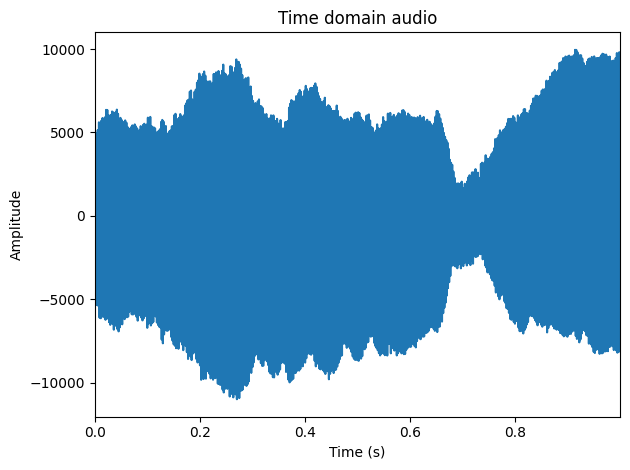
\includegraphics[width=\linewidth]{figs/time_domain_violin.png}
%  \caption{One second time domain violin sample.}
%  \Description{One second time domain violin sample.}
% \end{figure}

% \begin{figure}[h]
%  \centering
%  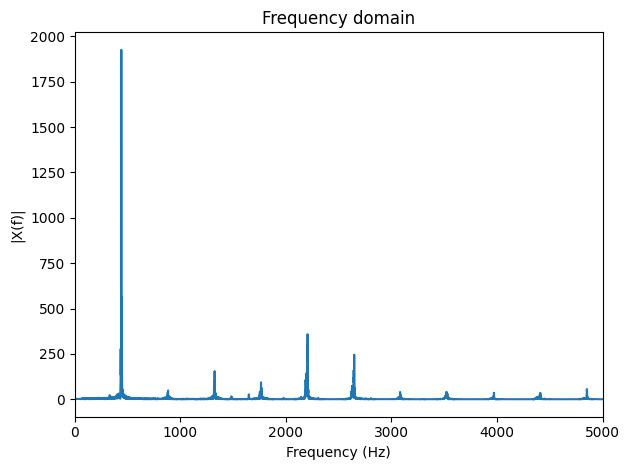
\includegraphics[width=\linewidth]{figs/frequency_doimain_violin.png}
%  \caption{The same one second frequency domain violin sample.}
%  \Description{One second frequency domain violin sample.}
% \end{figure}

% As the figures show, there is a main frequency that defines the pitch of the sound, along with many other frequencies that allow the ear to identify the instrument and distinguish between different kinds of sounds.

\subsection{Audio digitization}

A microphone can convert a pressure wave into an electrical waveform. However, in computational music, the audio signal must be discretized to be represented as a digital audio file.

% The primary process for digital audio representation is sampling.

To digitize an audio signal, a process called sampling is used (\textcite{po2022sampling}), which consists of recording a sequence of wave amplitudes at fixed time intervals. For human hearing, a sampling frequency of 20 kHz is generally sufficient, and, more specifically for music digitization, 16 kHz is often adequate (since even one of the highest-pitched instruments, such as the violin, reaches only around 3,500 Hz).

% For example, if a sound is recorded using a sampling rate of 22,100 Hz, it means that the computer will capture 22,100 audio samples per second.

% \begin{figure}[h]
%  \centering
%  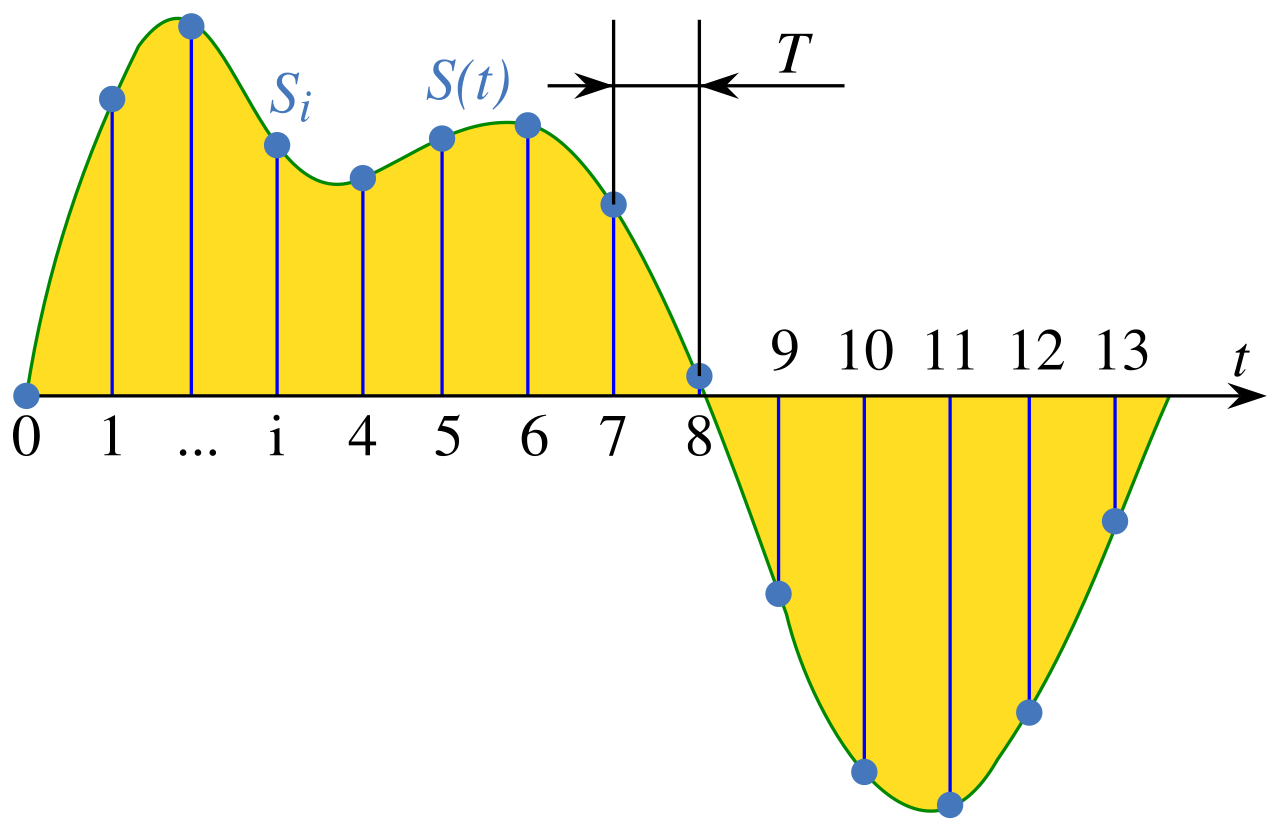
\includegraphics[width=\linewidth]{figs/signal_sampling.png}
%  \caption{Signal sampling. Source: Wikimedia Commons, \textit{Sampling (signal)}, CC BY-SA 4.0. \parencite{wikipedia_sampling}}
%  \Description{Sinal sampling.}
% \end{figure}

% This approach is highly efficient because human hearing can detect frequencies ranging from 20 Hz to 20,000 Hz (\textcite{benson2008music}). However, for most musical sounds, the maximum frequency is typically below 10 kHz; in fact, even a violin, one of the highest-pitched instruments, reaches only around 3,500 Hz. Thus, when considering only musical instruments, a 16 kHz sampling rate can be a reasonable choice for recording while saving disk space. Nevertheless, if the goal is to cover the full range of human hearing, higher rates such as 44,100 Hz can also be used.

%And according to the Nyquist-Shannon Theorem, to properly sample a periodic signal, the sampling rate must be at least twice the frequency of the highest component of the signal.

%Note that with this process, all sound elements highlighted before can be recorded and reproduced later.

%\subsection{Sound synthesis}

%After the development of sound recording techniques, musical computation evolved toward the creation of artificial waveforms. Of course, before digital audio synthesis, there were several techniques that allowed analog synthesis. However, the underlying idea is essentially quite similar.

%In summary, audio synthesis techniques can be divided into three basic types:

% Although there are many audio synthesis techniques, three of them represent the most direct forms of synthesis, or the most purely mathematical ones, in the sense that they do not require manipulation of pre-recorded audio. They are:

% %There are many other techniques that could be mentioned; however, these three represent the most direct forms of synthesis, or the most purely mathematical ones, in the sense that they do not require manipulation of pre-recorded audio.

% \begin{itemize}
%     \item \textbf{Additive synthesis:} Perhaps the most straightforward idea from a mathematical point of view. It consists of generating each frequency component of a desired timbre separately and then summing them. In fact, it is more like a weighted sum, since each component is weighted according to its contribution to the timbre. A normalization step is commonly applied after the process to avoid amplitude overload.

%     \item \textbf{Subtractive synthesis:} The opposite of the previous technique, but historically more common due to its effectivenessa and lower cost. In short, it consists of taking a complex waveform, rich in harmonics, and applying various filters to obtain the desired sound. It is more empirical than additive synthesis (which is based on spectral analysis), but simpler to implement and less computationally intensive. Typically, the original waveforms are complex ones such as the sawtooth wave, square wave, or triangular wave.

%     \item \textbf{FM synthesis:} Another empirical approach to sound synthesis, which will be addressed in detail in a later section. In short, it consists of altering a simple waveform by applying a high-frequency modulation, not to the generated waveform itself, but directly to the frequency parameter of the carrier oscillator. This type of distortion of the base frequency produces mirrored harmonics that enrich the sound's timbre. It is up to the musician to choose the appropriate parameters to produce the desired timbre.
% \end{itemize}

%There are many other techniques that could be mentioned; however, these three represent the most direct forms of synthesis, or the most purely mathematical ones, in the sense that they do not require manipulation of pre-recorded audio.

% \subsection{ADSR Audio envelop}

% Another important technique for achieving good results is the so-called “Attack, Decay, Sustain, and Release (ADSR) envelope”, which consists of applying a multiplicative function to the waveform, altering only its amplitude.

% The basic idea is to control the sound intensity by simulating the natural behavior of acoustic sounds. Typically, an ADSR envelope is defined as a function with a domain between 0 and 1, which is applied to the generated waveform:

% \begin{figure}[h]
%  \centering
%  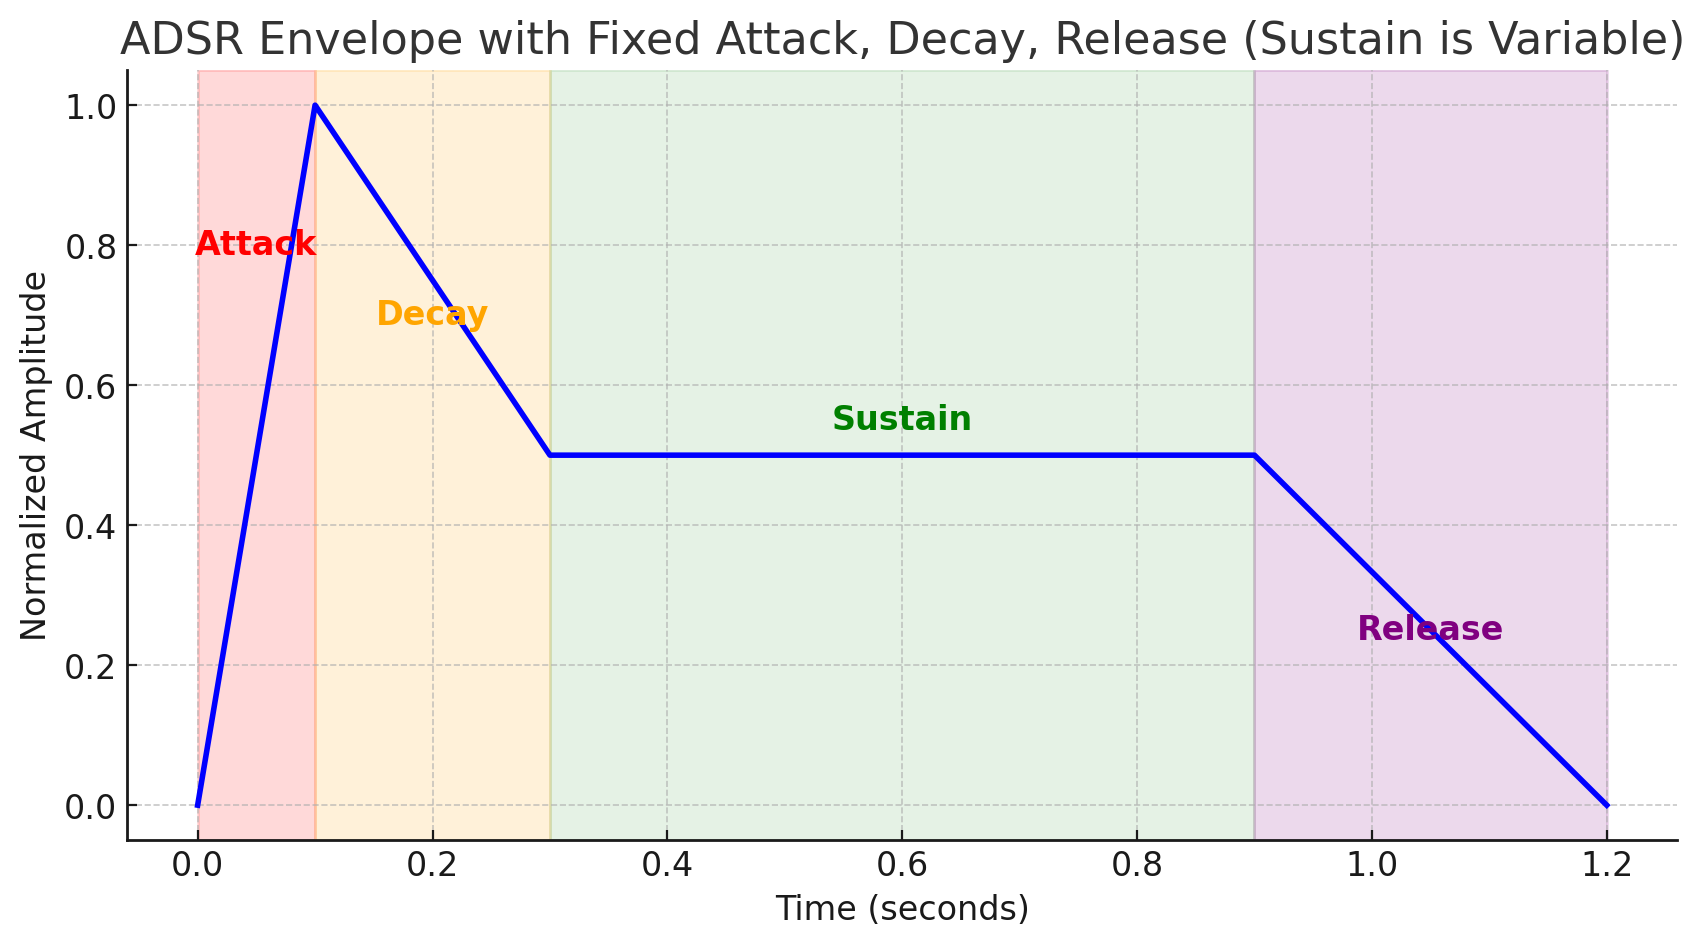
\includegraphics[width=\linewidth]{figs/adsr.png}
%  \caption{ADSR linear envelop.}
%  \Description{ADSR linear envelop.}
% \end{figure}

% The ADSR envelope can be understood as an amplitude function:

% \[
% y(t) = e(t) \cdot s(t)
% \]

% Where:

% \begin{itemize}
% \item \( s(t) \): the raw generated sound wave.
% \item \( e(t) \): the ADSR envelope function (normalized amplitude ranging from 0 to 1).
% \item \( y(t) \): the resulting sound.
% \end{itemize}

% Although real audio samples can show a wide variation of envelope behaviors, it is common practice to use a linear function to achieve the goal, since the human ear is more sensitive to abrupt changes and to relative differences. However, for long time variations, the ear can still perceive the change, which is why some synthesizers allow the use of exponential or logarithmic functions as well.

\subsection{Sound synthesis}
Although there are many audio synthesis techniques, three of them represent the most direct forms of synthesis, or the most purely mathematical ones, in the sense that they do not require manipulation of pre-recorded audio. They are:

%There are many other techniques that could be mentioned; however, these three represent the most direct forms of synthesis, or the most purely mathematical ones, in the sense that they do not require manipulation of pre-recorded audio.

\begin{itemize}
    \item \textbf{Additive synthesis:} Perhaps the most straightforward idea from a mathematical point of view. It consists of generating each frequency component of a desired timbre separately and then summing them (a weighted sum).

    \item \textbf{Subtractive synthesis:} The opposite of the previous technique, but historically more common due to its effectivenessa and lower cost. In short, it consists of taking a complex waveform, rich in harmonics, and applying various filters to obtain the desired sound (following an empirical workflow of trial and error).

    \item \textbf{FM synthesis:} Another empirical approach to sound synthesis, which will be addressed below.
\end{itemize}

%\subsection{FM Synthesis}

One of the most popular sound synthesis techniques is Frequency Modulation Synthesis (FM Synthesis), which was introduced by John M. Chowning~\cite{chowning1973synthesis}.% in his famous paper ``The Synthesis of Complex Audio Spectra by Means of Frequency Modulation'', published at the Stanford Artificial Intelligence Laboratory.
Chowning explored the effects of frequency modulation when applied with high frequencies, close to the audible range, instead of the traditional use of inaudible frequencies.

In summary, the FM synthesis technique allows the addition of multiple sidebands around the base frequency for each modulator used in the synthesizer algorithm. As a result, rich spectral audio can be created using only a few modulators, and a sound designer can, through an empirical process, create arbitrary sounds by adjusting the synthesizer parameters (\textcite{lazzarini2023higherorder}).

This type of synthesis was popularized by the Yamaha DX7 synthesizer and remains in use today due to its efficiency, low computational cost, and flexibility (\textcite{steinmetz2022ddx7}).

% In fact, the concept of frequency modulation was already well-known before this paper; however, it had been used mainly in radio transmission of music or to apply slight distortions through low-frequency oscillators (LFOs), producing effects such as vibrato.

% As Chowning himself pointed out in his paper, when the technique is applied to vary the frequency of the carrier wave through a high-frequency modulator wave, it ``results in a surprising control of audio spectra''.% (\textcite{chowning1973synthesis}).

% In summary, considering only two oscillators: the main one, called the carrier, and the modulator, the instantaneous frequency of the output audio can be expressed by the following function:

% \[
% f(t) = f_c + I \cdot \sin(2\pi f_m t)
% \]

% \noindent where:

% \begin{itemize}
% \item \( f(t) \): the instantaneous frequency of the generated sound wave.
% \item \( f_c \): the original frequency of the carrier wave.
% \item \( I \): the modulation index, which defines the intensity of the modulation (the greater the value, the more harmonics are generated).
% \item \( f_m \): the frequency of the modulator wave (which determines the spacing of the harmonics).
% \item \( t \): the time variable.
% \end{itemize}

% The most important point, however, is that this simple manipulation results in symmetric sidebands around the carrier frequency, spaced at multiples of \( f_m \).

% For a more intuitive understanding, if a carrier frequency \( f_m \) is modulated by a frequency \( f_m \), the resulting spectrum will contain:

% \[
% f_c \pm n f_m
% \]

% For example, by choosing \( f_c = 440 \) and \( f_m = 220 \), the resulting wave will contain frequency components such as 220 Hz, 440 Hz, 660 Hz, 880 Hz, and so on, with decreasing amplitudes (the amplitudes follow the Bessel coefficients, but this discussion is beyond the scope of this article).

% The last important characteristic of Frequency Modulation Synthesis concerns the ratio between the carrier frequency and the modulator frequency \( f_c / f_m \), since this ratio directly influences the perceived audio result.

% This ratio determines whether the generated harmonics align with the natural harmonic series (widely used by musicians) or not:

% \begin{itemize}
%     \item If the ratio is an integer number, the harmonic sidebands (in the spectral view) will appear as integer multiples of \( f_c \), generating harmonic sounds similar to those of real instruments (consistent with traditional music theory).
%     \item If the ratio is not an integer value, the harmonic sidebands will not align perfectly with \( f_c \), and the generated sound may appear metallic or dissonant (but, this effect is useful for creating sounds such as bells or for producing special audio effects).
% \end{itemize}

\subsection{Audio comparison}

The task of audio comparison is not straightforward, especially when the goal is to achieve perceptual similarity from a human hearing perspective. It can be complex, computationally demanding, and inherently subjective; however, several common and efficient methods can be employed to address this challenge. According to \textcite{claesson2021resynthesis}, the following methods can be highlighted.

% However, as described in the section on timbre, one intuitive and efficient way to approach this problem is by comparing the audio in its spectral representation, since timbre is precisely defined by this combination of frequencies.

% That said, this approach alone is not sufficient, because the Fourier Transform considers the entire audio signal at once, mixing different parts of a sound sample. For example, if a sample contains three different pitches in sequence, its frequency-domain representation will show them simultaneously, which may give the impression that the timbre is a mixture of all these pitches (similar to a chord rather than a sequence).

% In fact, according to \textcite{claesson2021resynthesis}, FFT-based spectral comparison is valid but only a part of the solution. He highlights the following metrics:

% According to \textcite{claesson2021resynthesis}, FFT-based spectral comparison is valid but only a part of the solution. He highlights the following metrics:

\begin{itemize}
    \item \textbf{FFT Distance:} This metric consists of computing the Fast Fourier Transform (FFT) of the two samples being compared and then calculating the Euclidean distance between them. The result can be normalized so that the maximum distance is 1 and the minimum is 0.
    \item \textbf{Short Time Fourier Transform (STFT) Distance:} Equivalent to the FFT Distance, but calculated over short, overlapping slices of the sample, which provides time-localized spectral information.
    \item \textbf{Log-Mel Spectogram Distance:} Similar to the previous metrics, but based on the Log-Mel Spectrogram, which is essentially an adaptation of the FFT spectrum that incorporates human auditory perception. In summary, the Log-Mel Spectrogram is obtained by computing the STFT, mapping the frequencies onto the Mel scale, which maps linear frequencies onto a logarithmic scale (\textcite{claesson2021resynthesis} and \textcite{chulev2024improving}).
\end{itemize}

In addition to these three metrics, \textcite{claesson2021resynthesis} also recommends the use of Euclidean Distance of the Envelope to compare audio envelopes. This approach can be very useful, but since this work is focused on the similarity between original and synthesized audio in terms of timbre, the envelope comparison, while important for real-world applications, falls outside the scope of the present study.

% \subsection{Mel-Scale Representation}

% The Mel scale was proposed by Stevens, Volkmann, and Newman in 1937 (\textcite{claesson2021resynthesis}), and its main purpose is to reflect the human perception of frequency.

% The key difference from the linear scale is that, as the values on the scale increase, the perceptual difference between two adjacent points becomes smaller.

% In fact, the Mel scale maps linear frequencies onto a logarithmic scale. A frequency \( f \) s converted to the Mel scale through the following formula:

% \[
% \text{Mel}(f) = 2595 \log_{10} \left( 1 + \frac{f}{700} \right)
% \]

% For a better understanding of this conversion, consider the following graph, which compares the linear hertz scale with the Mel scale:

% \begin{figure}[h]
%  \centering
%  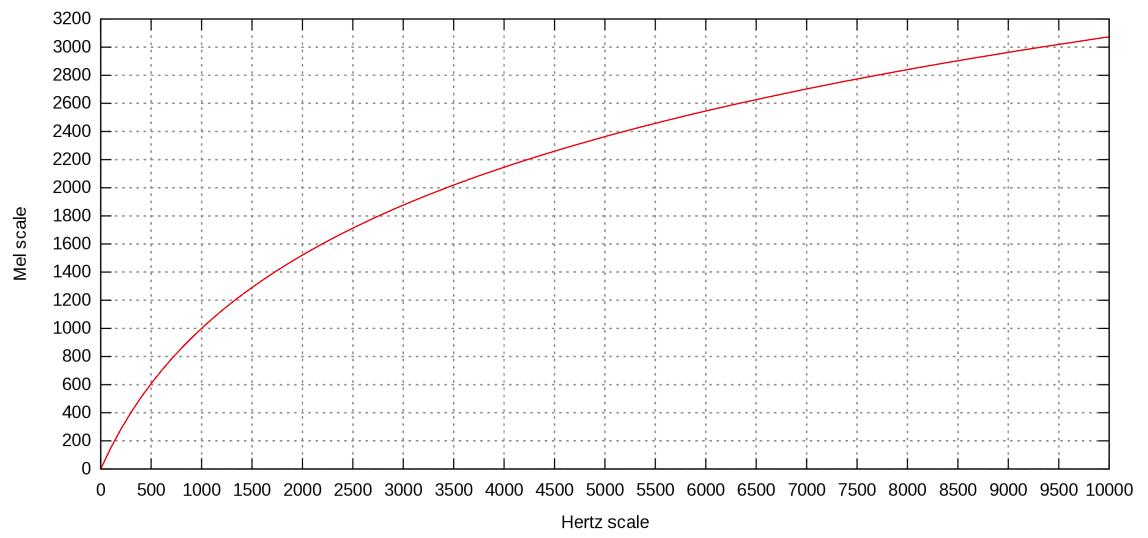
\includegraphics[width=\linewidth]{figs/mel_scale.png}
%  \caption{Comparision between linear hertz scale and Mel scale (\textcite{claesson2021resynthesis}).}
%  \Description{Comparision between linear hertz scale and Mel scale.}
% \end{figure}

% It is a very useful metric for audio comparison, as it takes into account the human auditory perception of frequency.

% \section{2D Convolutional Neural Networks (CNN)}

% %\subsubsection{2D Convolutional Neural Networks}

% In summary, a convolutional neural network is based on the idea of filters.

% Before the introduction of CNNs, was already known that many computer vision problems can be solved through the evaluation of image features, which become more evident depending on the filters applied.

% For exampe, to classify differe animals, just the silhouettes can be enough. Of course, the fewer features considered, the higher the chance of mistakes, but, as popular saying goes: “if it walks like a duck, quacks like a duck, flies like a duck… it’s a duck!”. That’s the basic idea.

% So, the CNNs were conceived in such a way that several layers of filters of fixed size (chosen by the network designer) are defined, in addition to some pooling layers (which will be discussed later).

% These filter layers are also organized according to the designer’s choices (usually based on many experiments) and can be applied in sequence, in parallel, using different combinations, and so on.

% However, it is essential to note that the filters serve as the link between the different representations of the input image built within the network.

% That is, although the network still takes an image as input, and although this image is processed to extract the various features needed for the problem, there are no dense interconnections between these image representations.

% In fact, what interposes between one image representation and another is precisely a CNN filter. And even this filter is not densely connected to the image representations.

% In practice, the filter is not connected to any specific part of the image. Instead, it is ``slid'' across the image, performing a Hadamard multiplication (element-wise product) between the filter and each frame of the image (of the same size), producing, as output, a ``new filtered image'' (multiplication, element by element, of two matrices of the same size, with a final sum of all elements — and, typically, with the application of an activation function to the result).

% Visually, the work can be represented as follows:

% \begin{figure}[h]
%  \centering
%  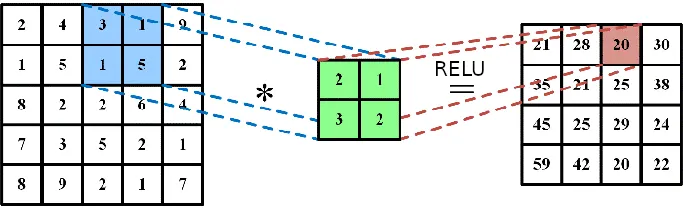
\includegraphics[width=\linewidth]{figs/hadamard_product.png}
%  \caption{Hadamard product between a filter and an input layer slice (adapted from \textcite{rokh2022hadamard})).}
%  \Description{Hadamard product between a filter and an input layer slice.}
% \end{figure}

% And it is precisely from this sliding operation that the network architecture derives its name, since this action corresponds to the mathematical operation of convolution, which can be viewed below:

% To an input image \( I \), a filter (or Kernel) \( K \), the convolution output \( O \), in a point \( (i,j) \) is given by:

% \[
% O(i,j) = \sum_{m=0}^{M-1} \sum_{n=0}^{N-1} K(m,n) \times I(i+m, j+n)
% \]

% Where:

% \begin{itemize}
% \item \( K(m,n) \): the filter element on position \( (m,n) \).
% \item \( I(i+m, j+n) \): the element of the input on position of current window.
% \item \( M, N \): the height and width of the filter.
% \item \( O(i,j) \): the output element on position \( (i,j) \).
% \end{itemize}

% Thus, CNNs can perform image filtering while at the same time reducing the amount of memory required compared to traditional fully connected feed-forward networks (because memory is allocated only for the filters and their results, rather than for each interconnection weight).

% After extracting the necessary features from the data, a small traditional dense (multi-layer) network is added in sequence to the convolutional (and pooling) layers. This dense network is responsible for identifying the patterns required to predict the target variable, whether for classification or regression tasks.

% A CNN is typically divided into two stages. The first stage consists of the application of filters (along with pooling layers), while the second stage applies a fully connected network. In this second stage, the output of the first part undergoes a flattening process, allowing it to be used as input to the fully connected layers, which perform the typical tasks of classification or regression.

\section{Related work} \label{sec:related}

It is not the first work to explore the idea of using a neural network to predict the appropriate parameters for a sound synthesizer. However, the main innovation here is the choice of CNNs to analyze the sound to be imitated. The main reasons are presented below:

\begin{itemize}
\item The ability of CNNs to process raw audio inputs.
\item The potential of CNNs to capture the temporal structure of sound samples.
\item The near real-time performance of CNNs, after training, which can be an advantage for future practical applications.
\end{itemize}

However, the following works were consulted to support this research and to guide the methodological comparison. The results, in fact, are difficult to compare due to the intrinsically different measurement scales:

\textcite{claesson2021resynthesis} proposed the re-synthesis of instrumental sounds using machine learning models combined with an FM synthesizer. However, \textcite{claesson2021resynthesis} did not use CNNs or the raw signal. Instead, he employed the STFT spectrogram as input (in other words, a frequency-domain representation of the signal), which may simplify the learning process but does not fully exploit the temporal information present in the audio.

\textcite{steinmetz2022ddx7} introduced DDX7, a differentiable FM synthesizer designed for the re-synthesis of musical instrument sounds. The strength of this work lies in the use of a type of CNN known as a Temporal Convolutional Network (TCN). However, their approach differs from the present work in terms of the chosen target values for the model. DDX7 operates directly on the Mel-spectrum representation, integrating it into the loss function. This was remarkable, as it provided the neural network with a loss function aligned with one of the most common audio comparison metrics. At the same time, this approach requires the synthesizer to be included in the training loop, which is more computationally expensive in terms of both memory and processing. Furthermore, compared with the present work, this research emphasizes the idea of strong generalization by generating a wide variety of parameter combinations through controlled random selection of FM parameters, as explained in the next section.

Finally, \textcite{kiranyaz2021survey} presented a comprehensive survey on 1D convolutional neural networks (CNNs) and their applications, highlighting their effectiveness in sequential data such as audio signals. Although this work does not focus on the same purpose (namely, the re-synthesis of audio samples), it explores various use cases for one-dimensional convolutional neural networks, including audio signal processing. This survey is an important reference that validates the applicability of CNNs to audio signals and their ability to capture the temporal structure of sounds.


\section{Methodology} \label{sec:our_proposal}

This section introduces our proposed approach of using AI to guide an FM synthesizer in simulating any instrument or any desired sound. More specifically, we propose a Convolutional Neural Network (CNN) to analyze a sound signal sample and predict the correct parameters for an FM synthesizer to re-synthesize the ``same'' timbre, enabling the synthesizer to simulate the desired ``voice'' playing any song. Since this idea is still quite abstract and broad, we consider the following steps:

\begin{enumerate}
    \item \textbf{Implementing FM synthesizer:} Implement a simple FM synthesizer, which can later be used both to generate the dataset and to test the ability to re-synthesize a sound.
    \item \textbf{Generating the dataset:} Generate an synthetic audio dataset composed of random samples, each created by randomly selecting FM synthesizer parameters. This essentially records tuples of (parameter values, audio sample) and explores the parameter space on a large scale.
    \item \textbf{Training the CNN:} Train a CNN to predict the correct parameters for the same FM synthesizer, given only an audio sample.
    \item \textbf{Evaluating the Model:} Evaluate the model's results using the NSynth dataset to test its generalization capabilities.
\end{enumerate}

Frequency Modulation Synthesis was chosen because it is one of the most common and effective methods for generating audio samples, owing to its simplicity and low computational cost.

This technique became extremely popular in the 1980s with the release of the Yamaha DX7 synthesizer. By the 1990s, it had become a standard for many commercial synthesizers and remains in use today in electronic music production (\textcite{claesson2021resynthesis}). However, the effective use of this technique depends on advanced knowledge to select the correct parameters for generating good results, which can involve thousands of parameters.

Therefore, the ability to simplify parameter selection constitutes a strong justification for this study, and AI models appear as an affordable way to learn the right patterns for controlling an FM synthesizer. The basic idea is that a model can be produced to guide an FM synthesizer in mimicking any sound, thereby optimizing the effort to compose electronic music.

Furthermore, in terms of computational cost, using an AI model to predict parameters and guide an FM synthesizer is much more effective than applying a Generative Neural Network to generate an audio. Additionally, a synthesizer is particularly well-suited for real-time composition and electronic musician performance.

Regarding the configuration aspects, all experiments were conducted in the following environment:

\begin{itemize}
    \item Python Version: 3.11.2
    \item Tensorflow Version: 2.19.0
    \item Keras Version: 3.11.1
    \item Nvidia-cuda Version: 12.5.82
    \item Nvidia-cudnn Version: 3.0.75
    \item Nvidia Driver Version: 535.247.01
    \item CUDA Version: 12.2
    \item GPU: NVIDIA GeForce GTX 1650 (4GB memory)
\end{itemize}

\subsection{Implementing FM synthesizer}

There are several well-known FM synthesizers on the market, but most are not open-source. Additionally, commercial synthesizers often have a vast number of parameters that can be used to control the audio production process. For example, Native Instruments' FM8 can use around 1,000 parameters (\textcite{claesson2021resynthesis}), and Teenage Engineering’s OP-1 synthesizer can be configured with up to $10^{76}$ parameters (\textcite{claesson2021resynthesis}).

This incredibly large number of parameters is intended to give users fine-grained control over the generated audio, allowing for a wide variety of pitches (simulating a broad range of instruments and even non-instrument sounds, such as bird songs or car horns, among others). However, since the scope of this project is not focused on a commercial solution but rather on research purposes, a simple FM synthesizer will suffice.

\begin{figure}[h]
    \centering
    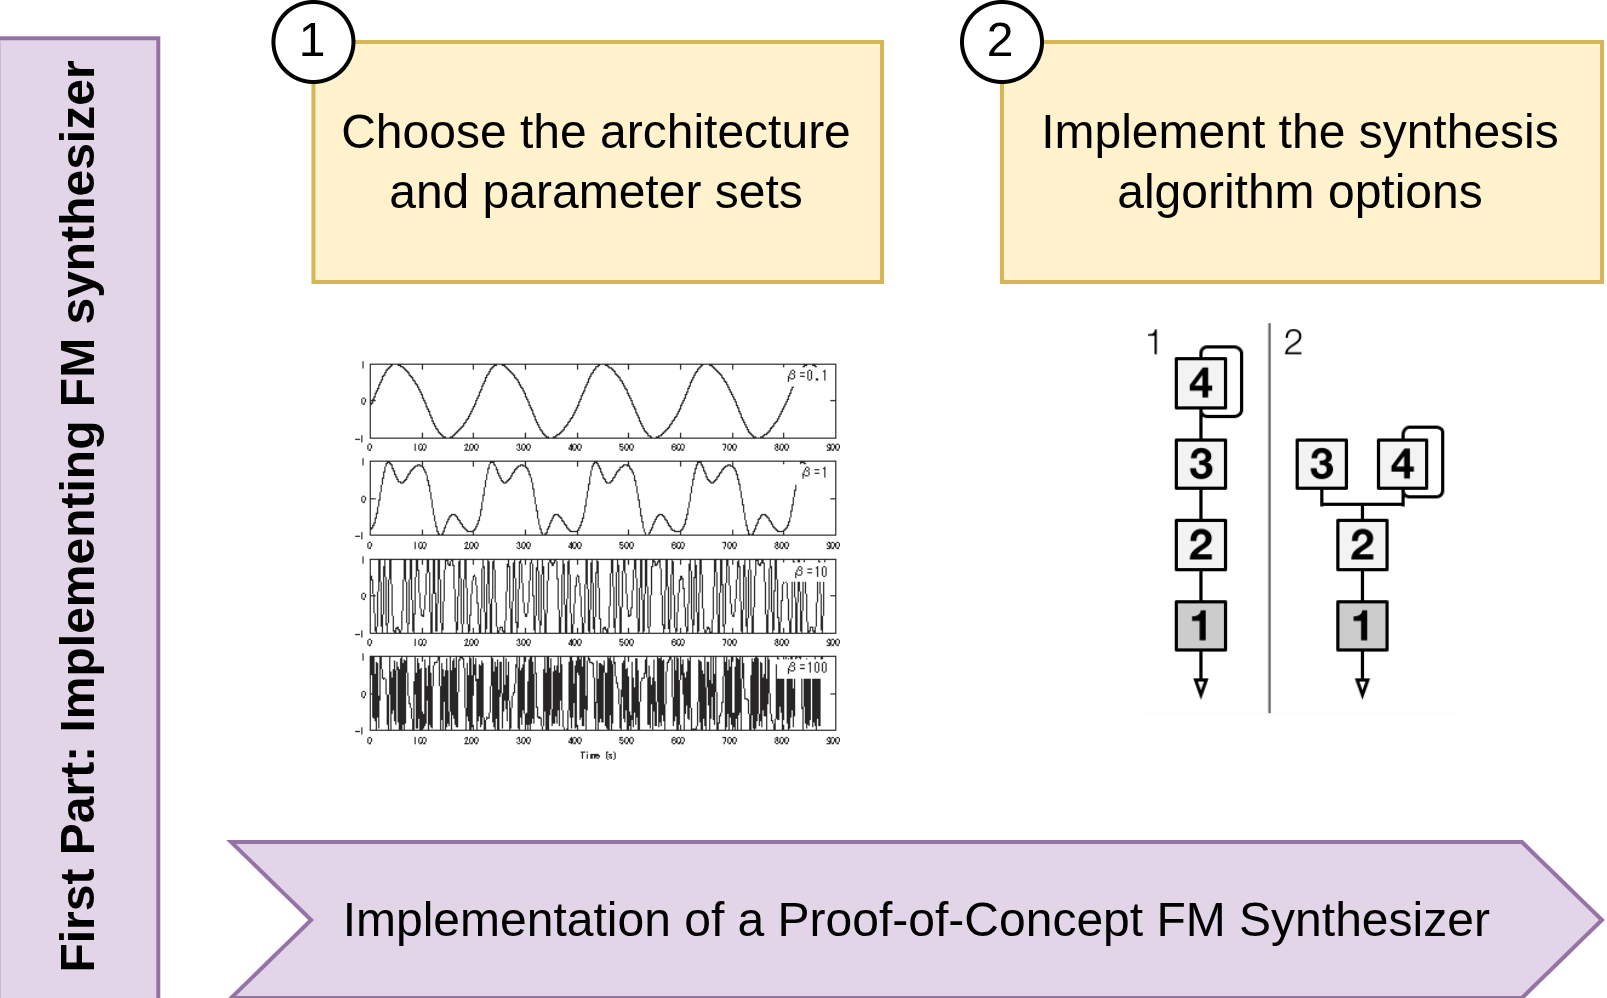
\includegraphics[width=1\columnwidth]{figs/first_part.png}
    \caption{Synthesis implementation and dataset generation.}
    \label{fig:met1}
\end{figure}

Therefore, this work will implement a basic FM synthesizer with only 6 operators, inspired by the classic Yamaha DX7, which was one of the most disruptive milestones in the history of electronic music composition. In fact, this simple setup is enough to cover all FM synthesis theories and achieve good performance during AI model evaluation. In summary, the implemented FM Synthesizer (Figure~\ref{fig:FMSynth}) consists of 5 modulator operators, 1 carrier operator, 1 ADSR envelope, and 2 synthesis algorithms (one completely serial, and another with 3 serial operators followed by 2 parallel operators).

\begin{figure}[h] 
    \centering
    \includegraphics[width=.9\linewidth]{figs/algs.png}
    \caption{FM Synthesizer Algorithms.}
    \label{fig:FMSynth}
\end{figure}

% \begin{itemize}
%     \item 5 modulator operators.
%     \item 1 carrier operator.
%     \item 1 ADSR envelope.
%     \item 2 synthesis algorithms (one completely serial, and another with 3 serial operators followed by 2 parallel operators).
% \end{itemize}

%The synthesizer will be implemented in Python, using the NumPy library for numerical processing and the SciPy library for audio file generation (in addition to the python-soundfile library).

%The figure below presents the FM Synthesizer algorithms:

To summarize, the implemented synthesizer renders the audio signal according to the following steps:

\begin{enumerate}
    \item Generate each operator signal by applying it to modulate the phase of the next operator in the sequence. In this implementation, only the phase is varied (similar to the Yamaha DX7), whereas a full FM synthesis would also be able to vary the frequency. This simplification helps to avoid complex noise-handling issues and promotes numerical stability. All signals are rendered at a 48 kHz sample rate.
    \item Combine the output of each operator according to the synthesis algorithm (when there are parallel operators, they are summed).
    \item Apply the ADSR envelope to the signal.
    \item Downsample the signal from 48 kHz to 16 kHz (applying also a low-pass filter to avoid aliasing).
\end{enumerate}

It is important to highlight that the high sample rate of 48 kHz was chosen to allow the FM synthesis to work well enough, since at high frequencies, there is a risk of obtaining aliasing and noise (due to the extremely high frequency components generated by the normal spacing of the FM operators). Furthermore, the low-pass filtering, used to downsample, is also useful to prevent the aliasing problem (after the downsampling process).

Finally, it is important to highlight that the entire synthesizer relies on 16 input parameters, consisting of the beta and ratio values for each modulator and for the carrier (totaling 12 parameters), plus 4 parameters for the ADSR envelope (attack, decay, sustain, and release times). As mentioned earlier, it is a very simple FM synthesizer, yet fully featured and sufficient for the purposes of the current research.

\subsection{Generating the dataset}

This work utilizes two datasets, each serving a distinct purpose: the generated dataset, referred to below as the synthetic dataset, which is used for training, and the NSynth dataset, which is used to evaluate the model’s generalization capabilities. However, in this section, only the first dataset will be considered, while the second will be addressed in the Section~\ref{sec:evaluation_method}.

One of the most challenging steps in the KDD process is obtaining and processing data. However, for the purposes of this work, an effective approach can be used. Similar to Claesson's approach (\textcite{claesson2021resynthesis}), since the goal is to achieve good control over the synthesizer parameters, it is sufficient to generate many samples of synthesizer parameters and their respective audio outputs.

\begin{figure}[h]
    \centering
    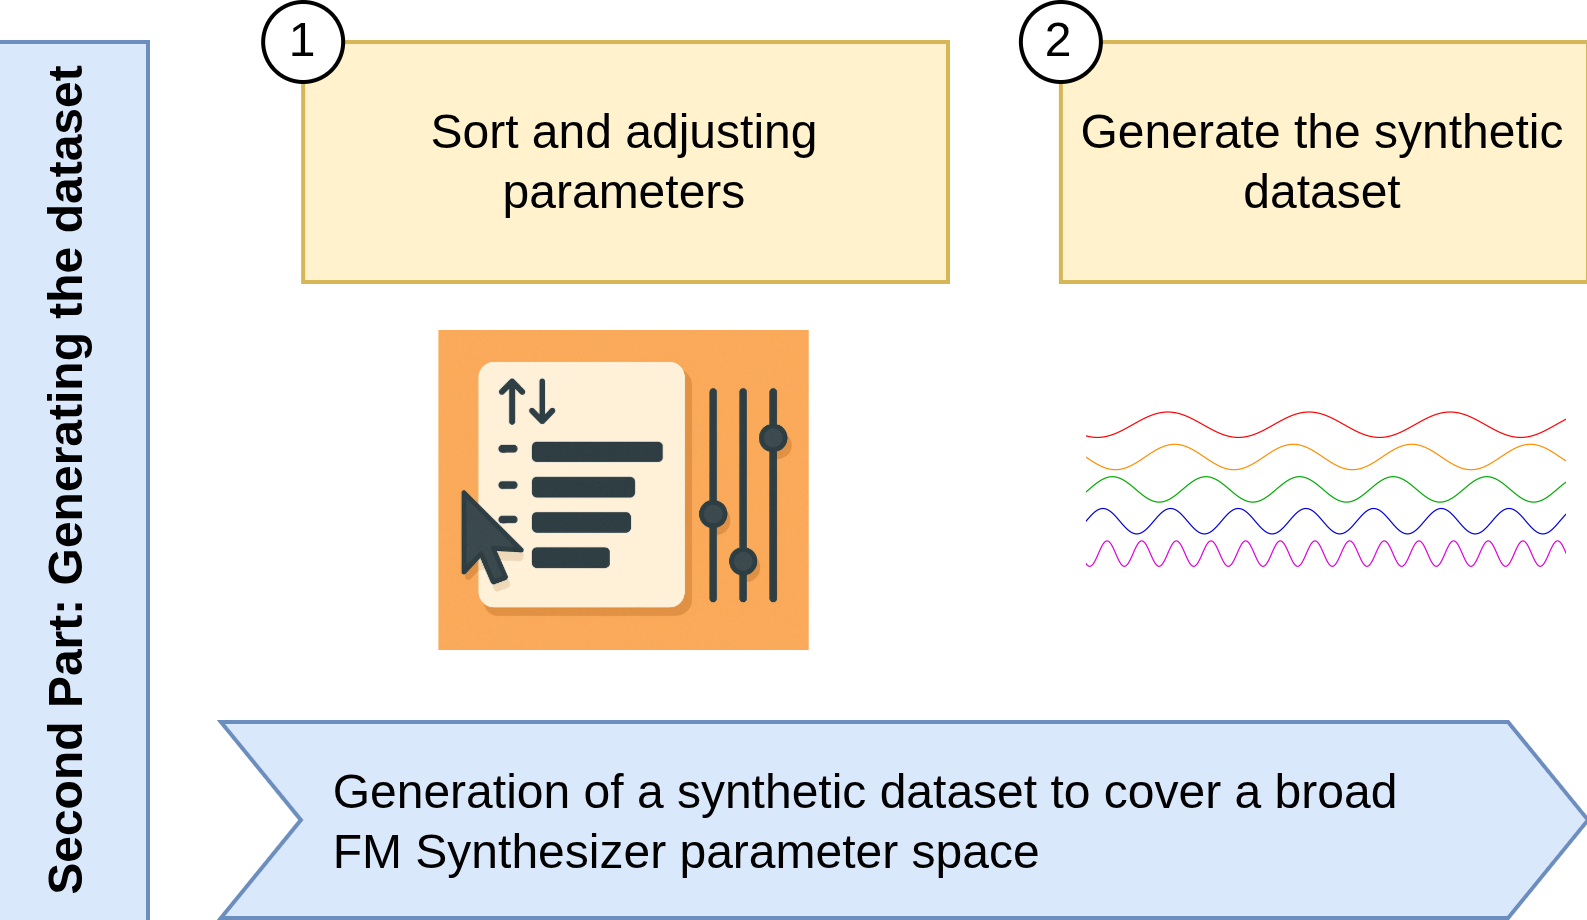
\includegraphics[width=1\columnwidth]{figs/second_part.png}
    \caption{Synthesis implementation and dataset generation.}
    \label{fig:met1}
\end{figure}

The dataset used to train the model will consist of 5,000 samples generated by the implemented FM synthesizer, with the following characteristics:

\begin{itemize}
    \item 5,000 samples.
    \item 4 seconds in duration.
    \item Monophonic samples (1-channel audio).
    \item 16 kHz audio sample rate (the synthesizer will generate samples at 48 kHz, but they will be downsampled to 16 kHz, to be compatible with the NSynth dataset).
    \item Pitches varying between 20 Hz and 6,000 Hz.
    \item Random ADSR envelopes.
\end{itemize}

The expectation is to achieve a level of learning where the model can accurately predict the parameters for a wide range of sounds that can be generated by the implemented FM synthesizer.

However, as the main purpose is to re-synthesize real instruments samples, the randomness of this dataset should be controlled to achieve reasonable music property samples, or, in other words, the dataset was constructed respecting the well-known limits and characteristics of real instruments:

\begin{itemize}
    \item The minimum frequency for the carrier is 20 Hz, and the maximum is 6 kHz (for example, the maximum frequency for a violin is approximately 3 kHz; another important aspect for this maximum choice is that we need to stay under 8 kHz due to the output sample rate, because of the Nyquist frequency). The frequency is chosen by a uniform random distribution.
    \item The minimum ratio for each modulator is 1/8, and the maximum is 8 (to avoid aliasing in the final signal). Two methods are used to select the ratio: a) with 90\% probability, the ratio will be a random uniform choice between discretized values (for example: 1/8, 1/6, ..., 2, 3, 54, ..., 8; the idea is to simulate a real instrument); and b) with 10\% probability, the ratio will be a uniform log distribution between 1/8 and 8 (allowing random metallic sounds, like bells, but respecting human auditory perception, where the difference between low frequencies is more perceived than between high frequencies).
    \item The minimum beta is 0, and the maximum is 8 (also to avoid aliasing in the final signal). The beta is chosen by a uniform random distribution, controlled such that 20\% of the values are between 0 and 0.5, 60\% are between 0.5 and 3, and 20\% are between 3 and 8 (prioritizing rich timbres and avoiding pure sinusoidal sounds, as well as excessive metallic sounds).
    \item The amplitude is fixed at 1.0, to avoid different combinations of beta and amplitude generating the same frequency spectrum and the same timbre (prioritizing the CNN learning).
\end{itemize}

About the ADSR envelope, the following adjustments were made:

\begin{table}
  \caption{Random Uniform ADSR Time Intervals}
  \label{tab:time_intervals}
  \begin{tabular}{cl}
    \toprule
    Parameter & Interval \\
    \midrule
    Attack  & [0.005, 0.5] \\
    Decay   & [0.02, 0.6] \\
    Sustain & [0.1, 0.9] \\
    Release & [0.05, 0.8] \\
    \bottomrule
  \end{tabular}
\end{table}

With these additional adjustments, the synthetic dataset will be more representative of simulating real instruments.

As each sample in the generated dataset is a complete 4-second sound (containing 64,000 audio samples, which corresponds to 16 kHz multiplied by 4 seconds), so a simple 75/25 train-test split was used, resulting in 3,750 audio files for training and 1,250 for testing.

But, from these 3,750 audio files, 20\% of them will be used for validation, resulting in a total of 3,000 samples for training and 750 samples for testing.

\subsection{Training the CNN}

As described in Section~\ref{sec:fund}, the main characteristic of the sound that should be reproduced to achieve the main work goal is the ``timbre``, which is defined as the combination of frequencies present in the sound. It is clear that techniques such as filtering and Fourier Transform can be used to extract timbre components from an audio signal; however, they are insufficient for controlling an FM Synthesizer. In fact, the FM Synthesis control is, normally, an experimental process involving trial and error.

Additionally, each FM Synthesis operator generates additional frequency components in the signal, and there is no practical method to predict the correct parameter settings. However, as a mathematical function, it is easy to see that this synthesis pattern can be easily approximated using AI models.

Thus, the current work aims to use a CNN model, since it is a very effective method for learning patterns, respecting the internal data structure, and without requiring extensive preprocessing work. In other words, a CNN can simultaneously learn the time-dependent aspects of an audio signal and can act as a pattern extractor by applying a sequence of filtering operations, allowing the use of the raw audio format as input.

To train the CNN model, the already presented synthetic dataset will be used. Its main advantage is that it contains both the audio signal and the corresponding parameters used to generate each sample. In addition, this approach covers a wide range of the parameter space.

Consequently, the training process is straightforward and is expected to yield good performance.

Figure~\ref{fig:met2} presents the overall scheme of this training process.

\begin{figure}[h]
    \centering
    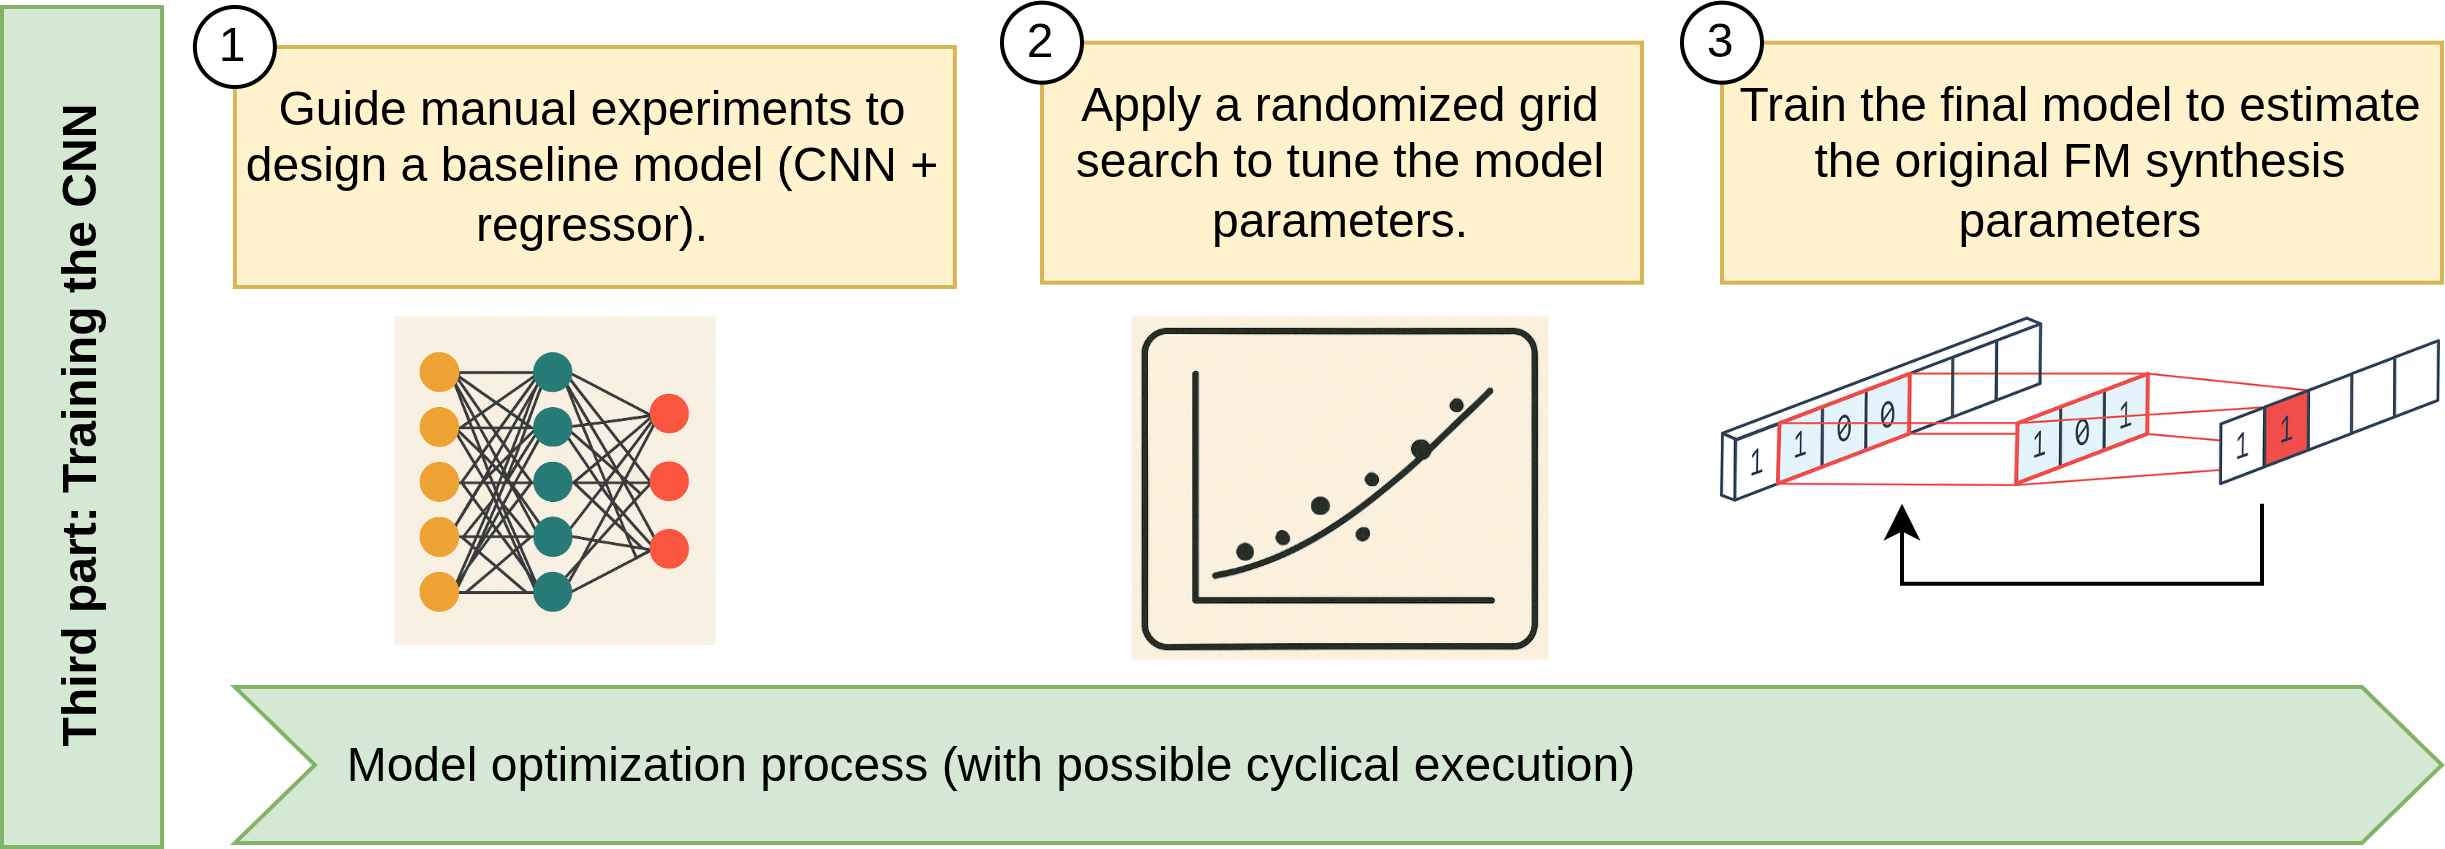
\includegraphics[width=1\columnwidth]{figs/thrid_part.png}
    \caption{Model training and optimization.}
    \label{fig:met2}
\end{figure}

The model architecture used is as follows, where the first covers the feature extraction (CNN), and the second covers the regression (a common MLP):

\begin{figure}[h]
    \centering
    \subfloat[][Feature extration]{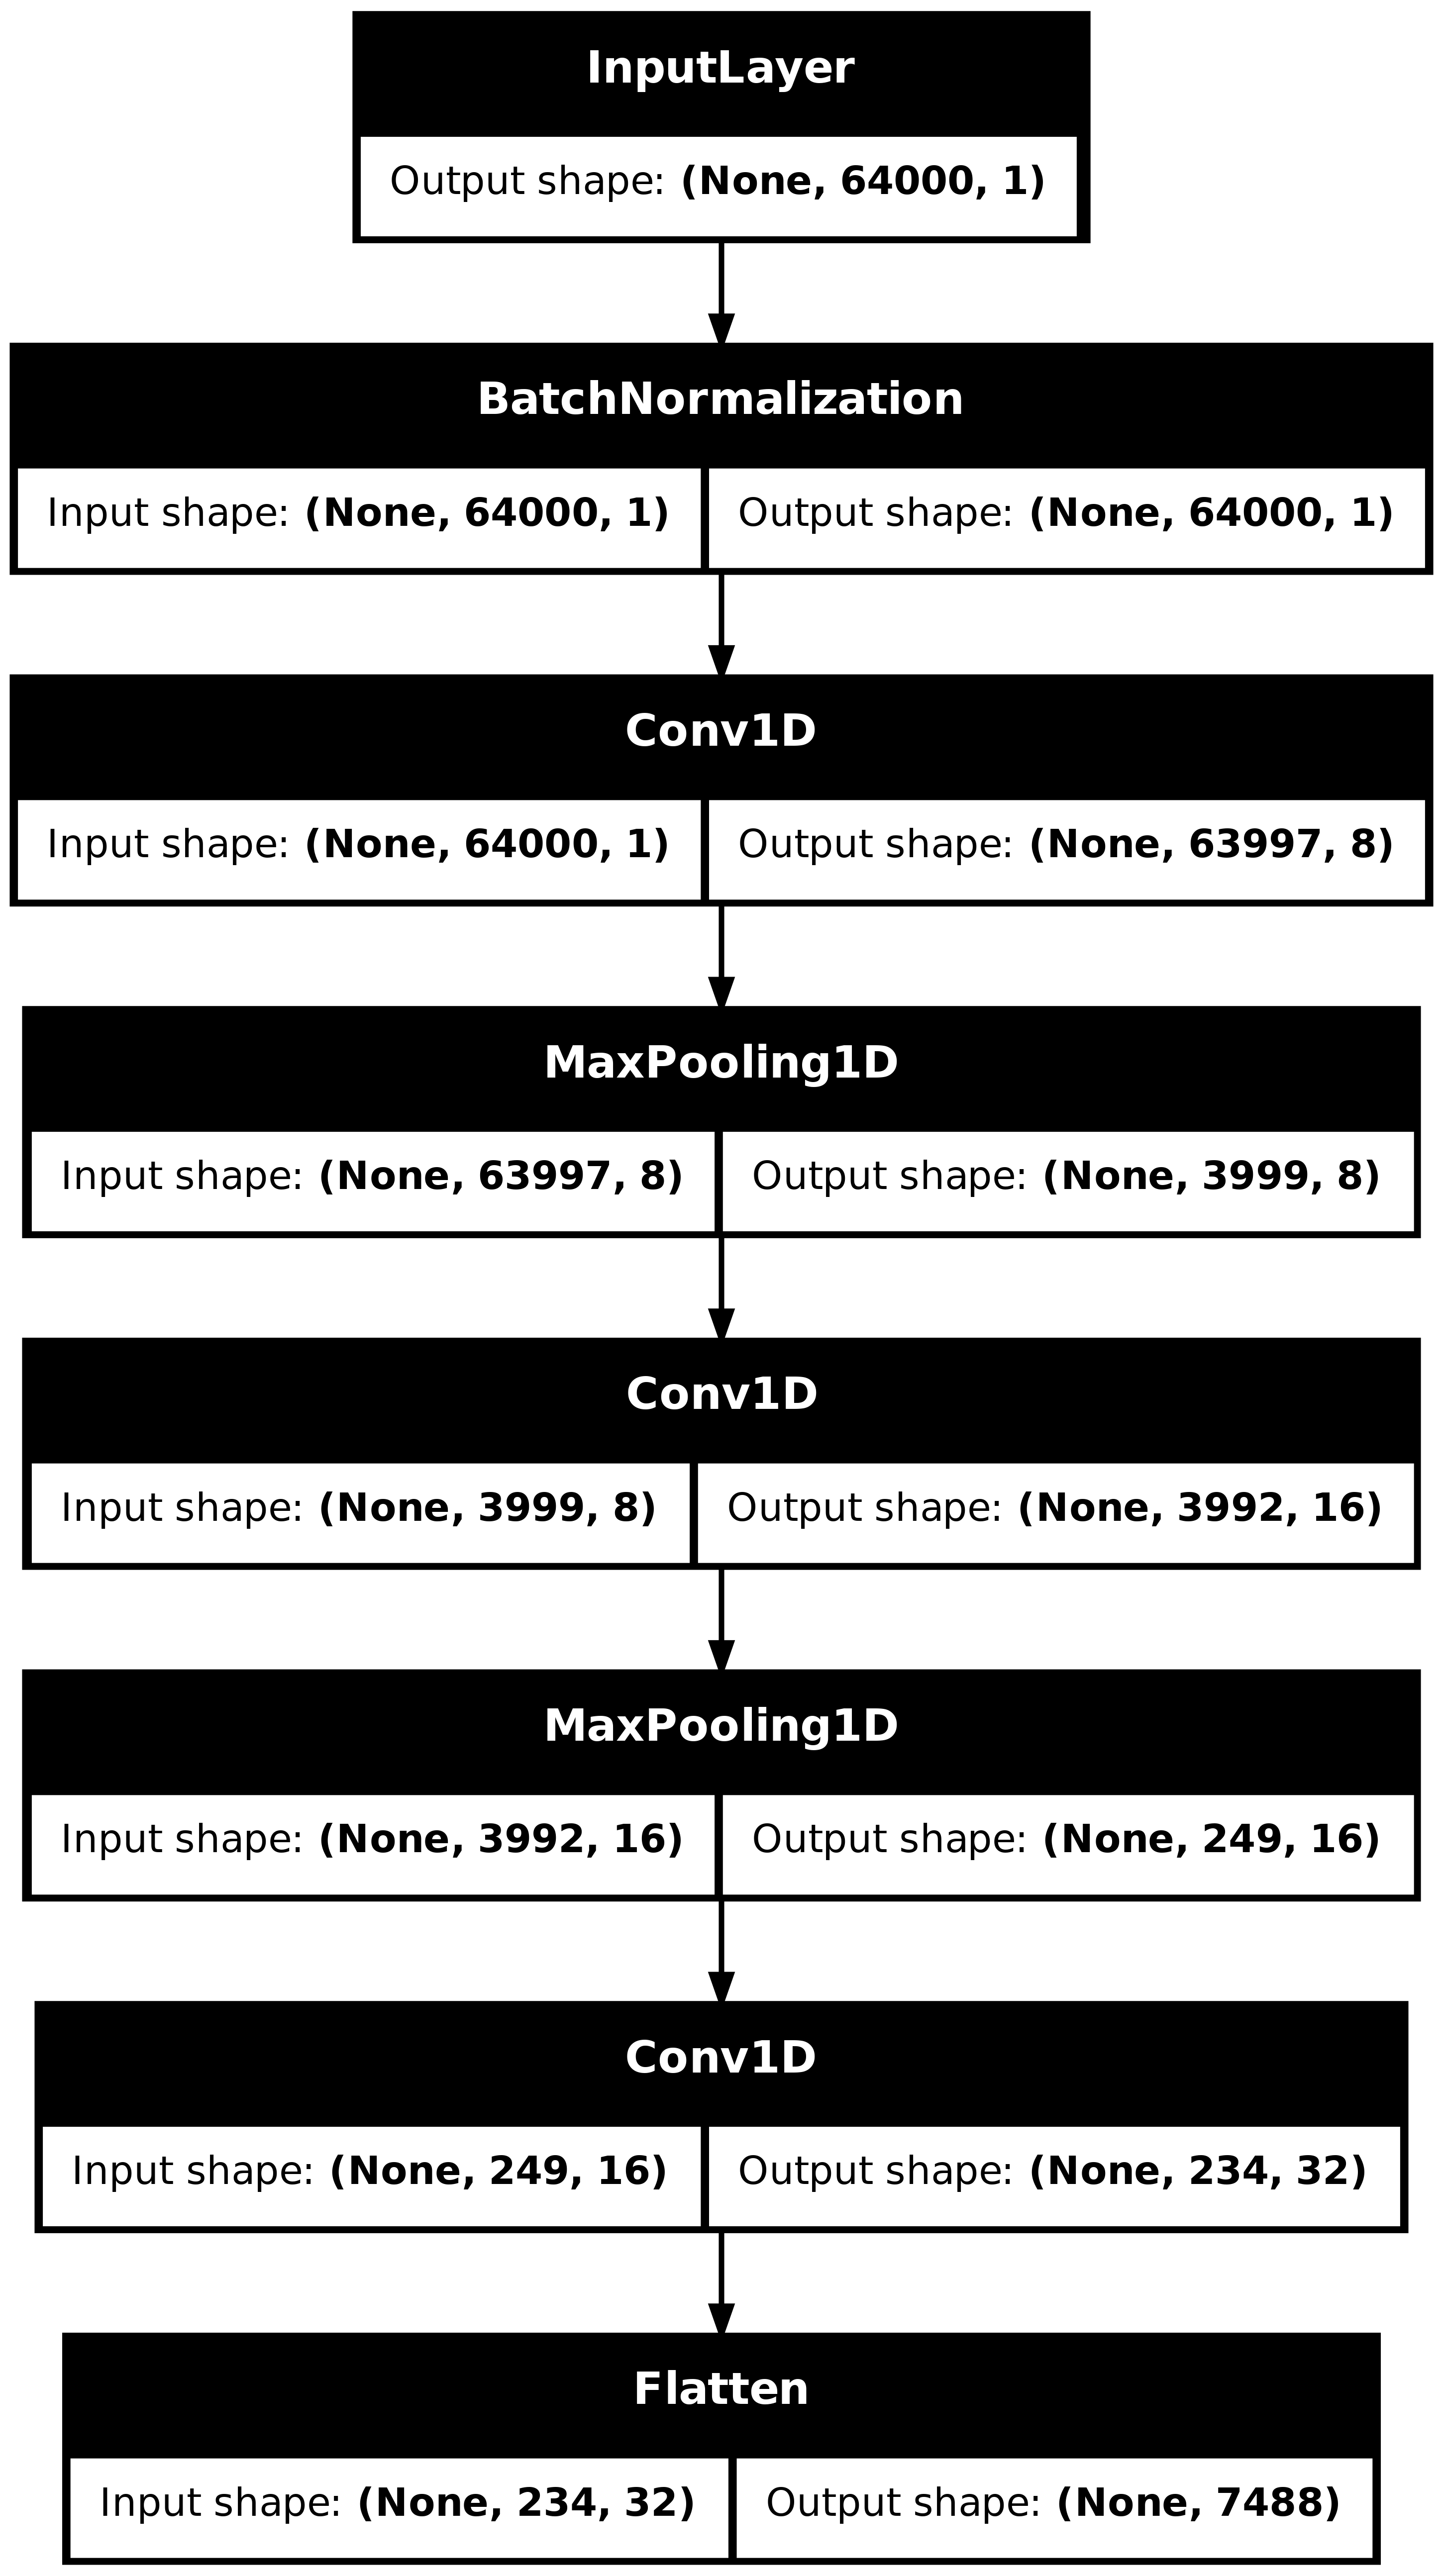
\includegraphics[width=0.21\textwidth,height=0.4\textwidth,trim={0 0 0 0.6cm},clip]{figs/rede1.png}} \label{fig:rede1}
    \qquad
    \subfloat[][Regressor]{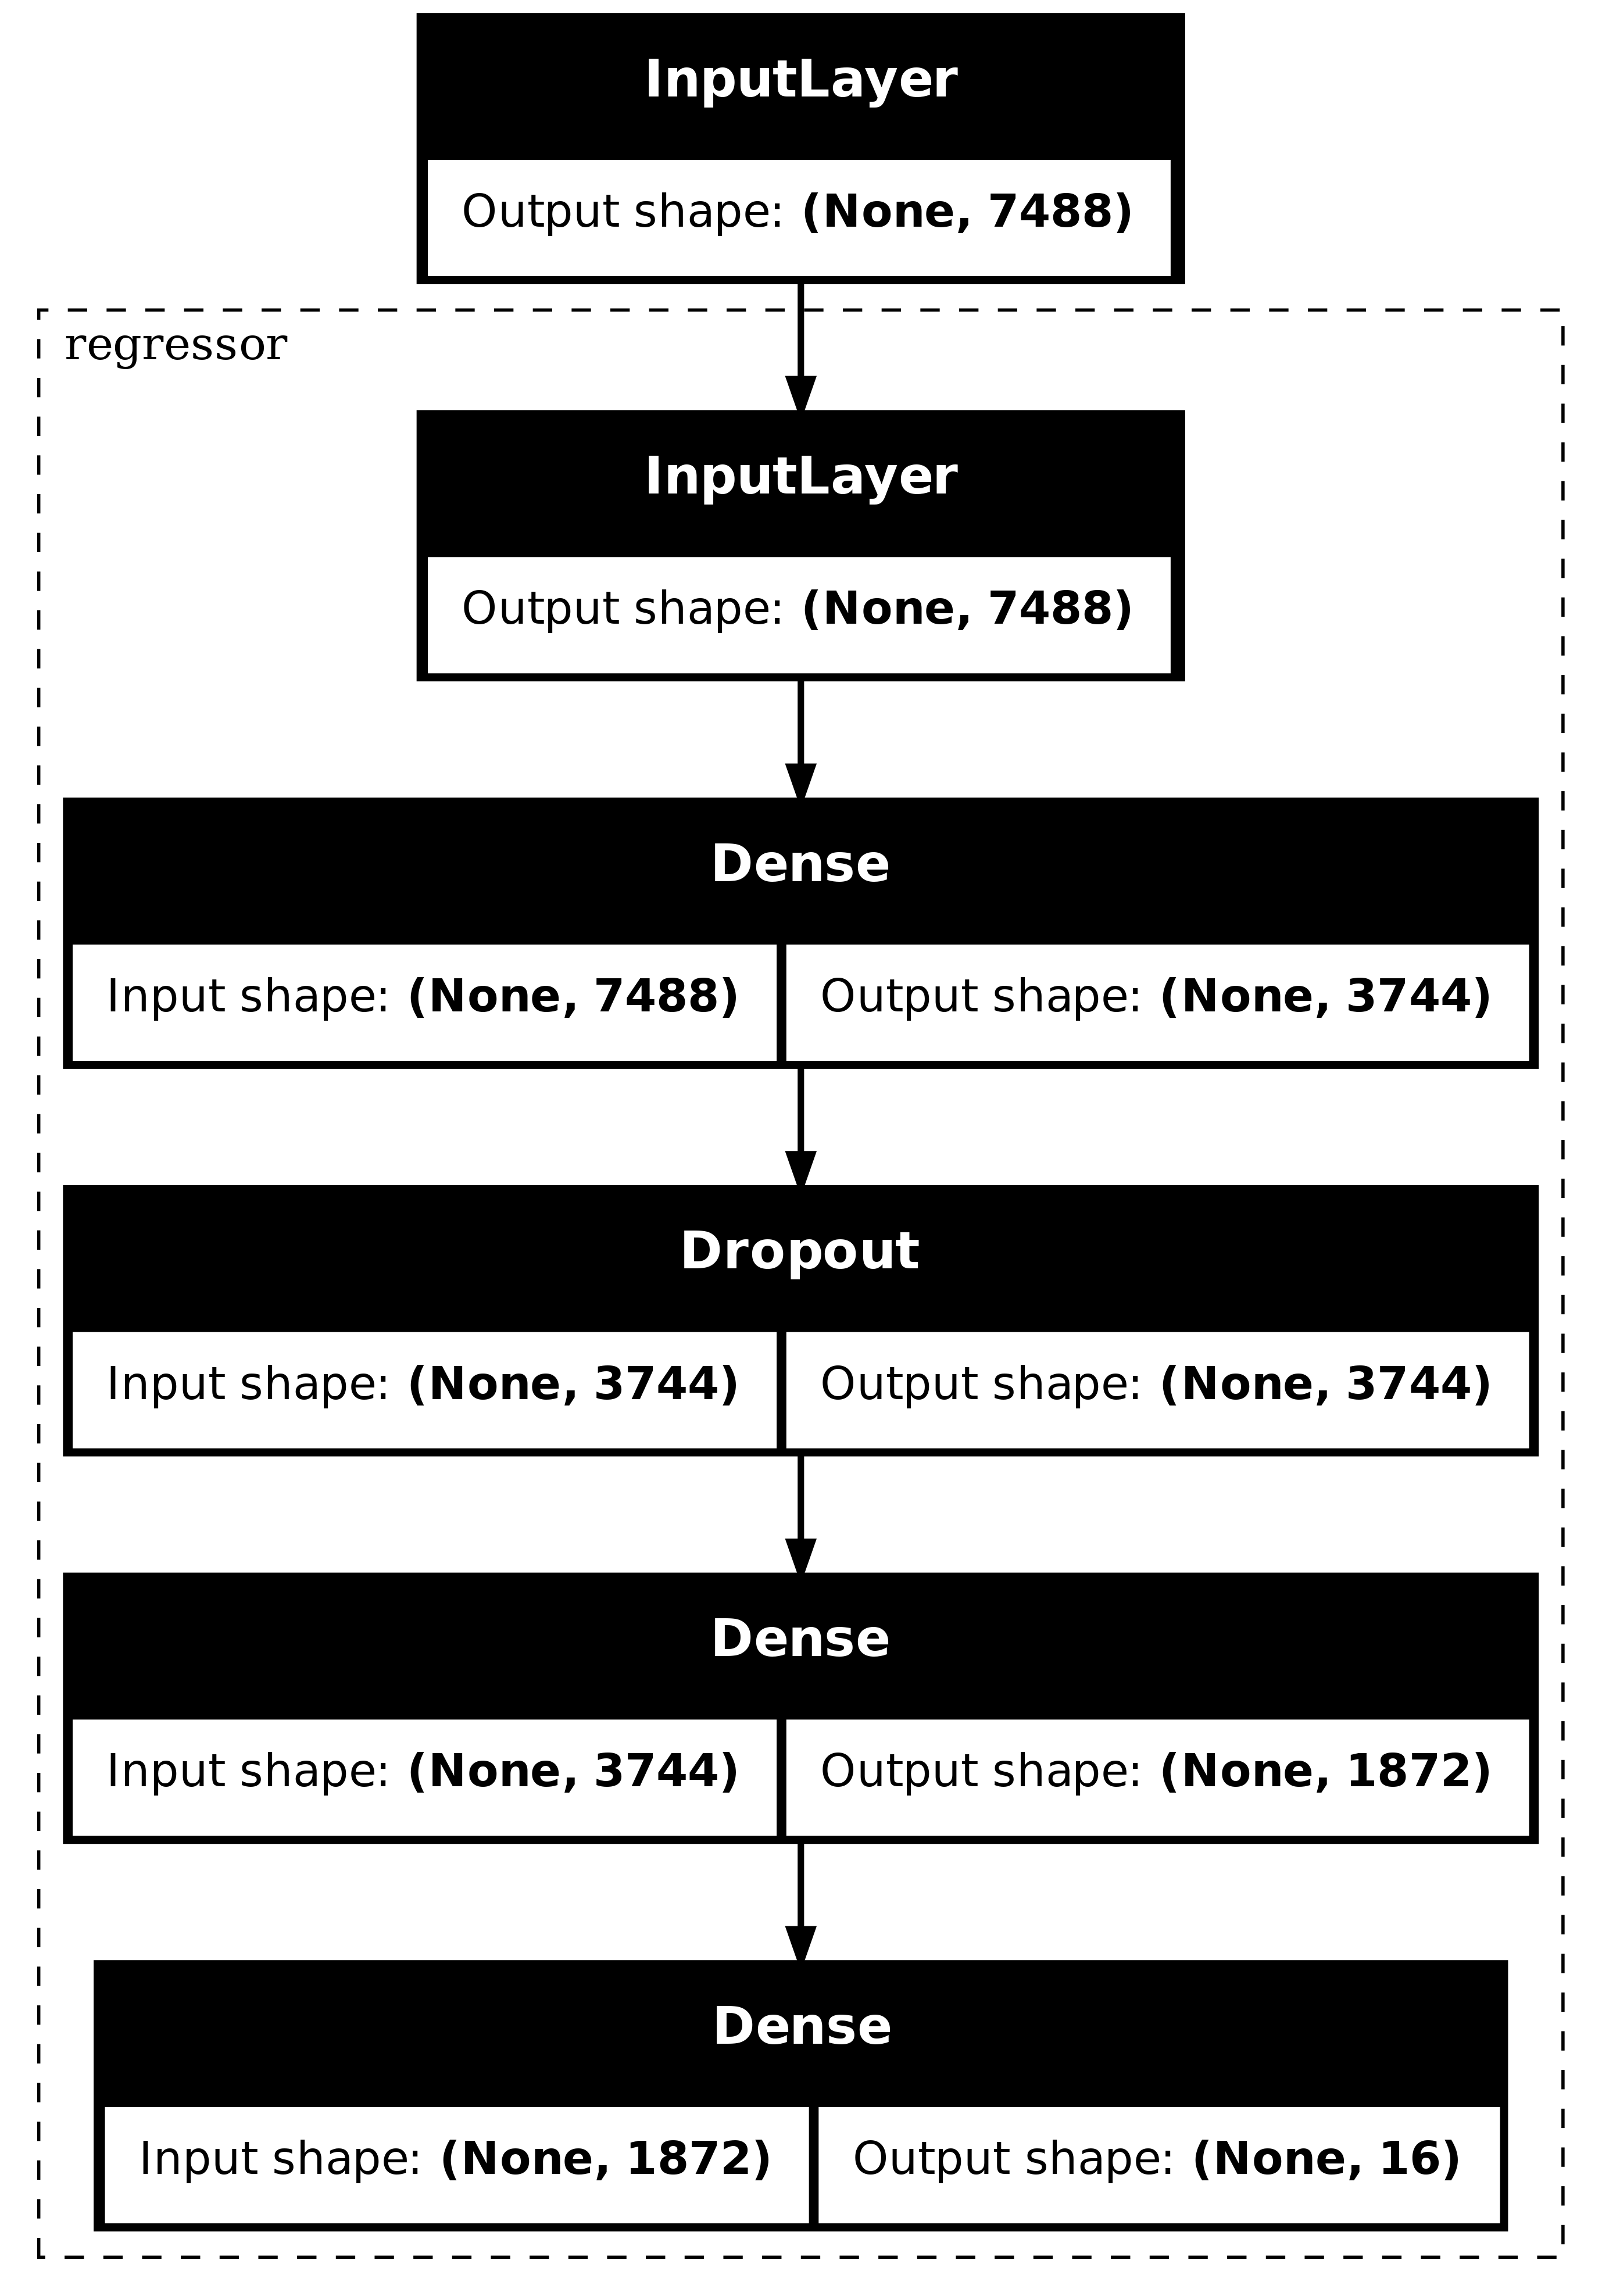
\includegraphics[width=0.21\textwidth,height=0.4\textwidth,trim={0 0 0 0.85cm},clip]{figs/rede2.png}} \label{fig:rede2}
    \caption{Overview of the entire Model Architecture}
    \label{fig:redes}
\end{figure}


The complete model is simply the sum of the two parts. But it is important to highlight the hyperparameters of each part:

\begin{table} \small
  \caption{Hyperparameters of Features Extraction (CNN part)}
  \label{tab:hyperparams_cnn}
  \begin{tabular}{cll}
    \toprule
    Component & Hyperparameter & Value \\
    \midrule
    \multirow{3}{*}{Conv1D (1)} 
        & Filters & 8 \\
        & Kernel size & 4 \\
        & Strides & 1 \\
    MaxPooling1D (1) & Pool size & 16 \\
    \multirow{3}{*}{Conv1D (2)} 
        & Filters & 16 \\
        & Kernel size & 8 \\
        & Strides & 1 \\
    MaxPooling1D (2) & Pool size & 16 \\
    \multirow{3}{*}{Conv1D (3)} 
        & Filters & 32 \\
        & Kernel size & 16 \\
        & Strides & 1 \\
    MaxPooling1D (3) & Pool size & 16 \\
    \bottomrule
  \end{tabular}
\end{table}


\begin{table} \small
  \caption{Hyperparameters of the Regressor Network}
  \label{tab:hyperparams_regressor}
  \begin{tabular}{cll}
    \toprule
    Component & Hyperparameter & Value \\
    \midrule
    \multirow{1}{*}{Dense (1)} 
        & Activation & relu \\
    Dropout & Rate & 0.5 \\
    \multirow{1}{*}{Dense (2)} 
        & Activation & relu \\
    \multirow{1}{*}{Dense (Output)} 
        & Activation & None \\
    Optimizer & -- & Nadam \\
    \bottomrule
  \end{tabular}
\end{table}

Other important highlights:

\begin{itemize}
    \item The target variable is normalized to have a mean of 0 and a standard deviation of 1, prior to training.
    \item The Nadam optimizer was used.
    \item The Mean Squared Error (MSE) was used as the loss function.
    \item The recorded metrics were the Mean Absolute Error (MAE), and the Mean Squared Error (MSE).
    \item The model was trained for 200 epochs, with early stopping enabled using 20 epochs of patience and best weights restoring.
    \item The model was trained with a batch size of 32.
\end{itemize}

\subsubsection{Hyperparameters Optimization}

To reach the previous defined architecture, after an initial phase of experiments aimed at selecting a generic architecture able to achieve the proposed goals, a grid search process was applied to optimize the model’s hyperparameters.

This grid search did not differ substantially from the traditional process, but it is important to highlight the search space and the chosen strategy to obtain a good representation of the parameter space without requiring exhaustive experimentation.

The following hyperparameters and their respective options were used:

\begin{table} \small
  \caption{Hyperparameters and Available Options}
  \label{tab:hyperparams_options}
\begin{tabular}{ll}
    \toprule
    Hyperparameter & Options \\
    \midrule
    Activation & gelu, swish, elu, relu, selu, silu \\
    Bias (CNN) & True, False \\
    Kernel Regularizer (CNN) & None, l1, l2 \\
    Bias (Regressor) & True, False \\
    Dropout (Regressor) & 0, 0.2, 0.3, 0.5 \\
    Kernel Regularizer (Regressor) & None, l1, l2 \\
    Optimizer & AdamW, RMSprop, Adam, \\
    -- & Nadam, Adagrad, Adamax \\
    \bottomrule
  \end{tabular}
\end{table}

However, calculating the total number of possible parameter combinations results in the remarkable value of 5,184 options. An exhaustive search over this space would take nearly nine days, given that 186 experiments required approximately seven hours.

To make the process viable, a random shuffle of the parameter search space was applied, producing a new order of experiments that did not require exhausting all options of a given parameter before moving on to the next.

Using this shuffled hyperparameter space, 186 experiments were conducted, representing nearly 3.6\% of the total and requiring about seven hours of training.

This approach enabled the representation of a generic sample of the entire search space within a feasible time frame. Since any parameter option could appear in the sampled configurations, the random grid search allowed for faster and broader coverage of the parameter space.

Furthermore, each combination was used to train for 30 epochs with an early stopping patience of 5. All tested hyperparameters and their respective error metric values were recorded using the MLflow tool, which enabled more accurate comparisons among the top solutions. This, in turn, helped guide the selection of good hyperparameters and supported a more targeted exhaustive training phase, already informed by the most successful configurations.

To provide a clearer understanding of this point, consider the following experiment comparison graph:

\begin{figure*}[h]
 \centering
 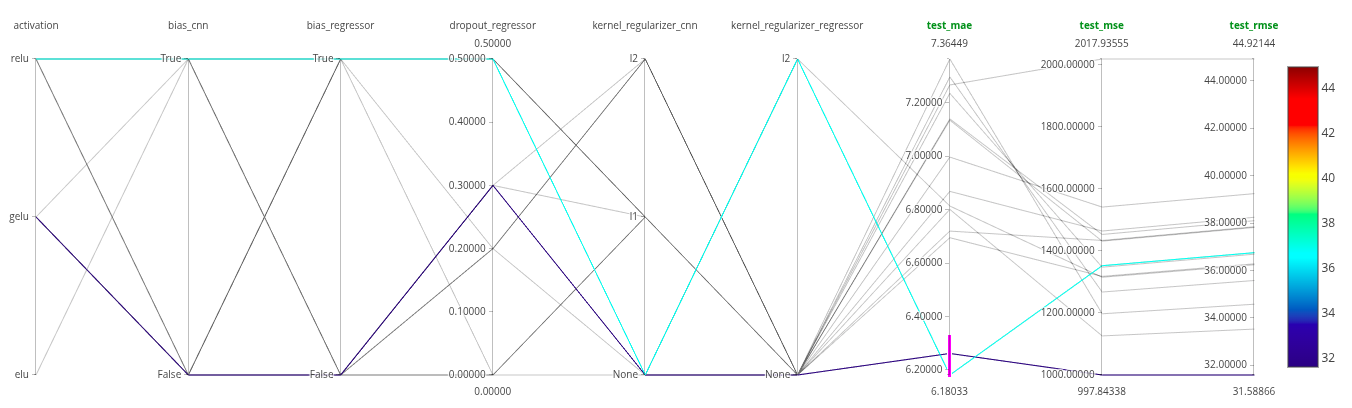
\includegraphics[width=.9\linewidth]{figs/graph_grid_search.png}
 \caption{MLflow grid search results showing the best error metrics (based on the test set).}
 \Description{MLflow grid search results showing the best error metrics.}
\end{figure*}

Note in the figure above that the following configurations appear successful, based on the three error metrics:

\begin{itemize}
\item \textbf{Activation function:} RELU
\item \textbf{CNN Bias:} True
\item \textbf{Regressor Bias:} True
\item \textbf{Regressor Dropout:} 0.5
\item \textbf{CNN Kernel Regularizer:} None
\item \textbf{Regressor Kernel Regularizer:} L2
\end{itemize}

It should be noted that the two best configurations, considering the MAE metric, were tested, and the second one (with respect to MAE) showed the best results without signs of overfitting.

% \begin{figure}[h]
%     \centering
%     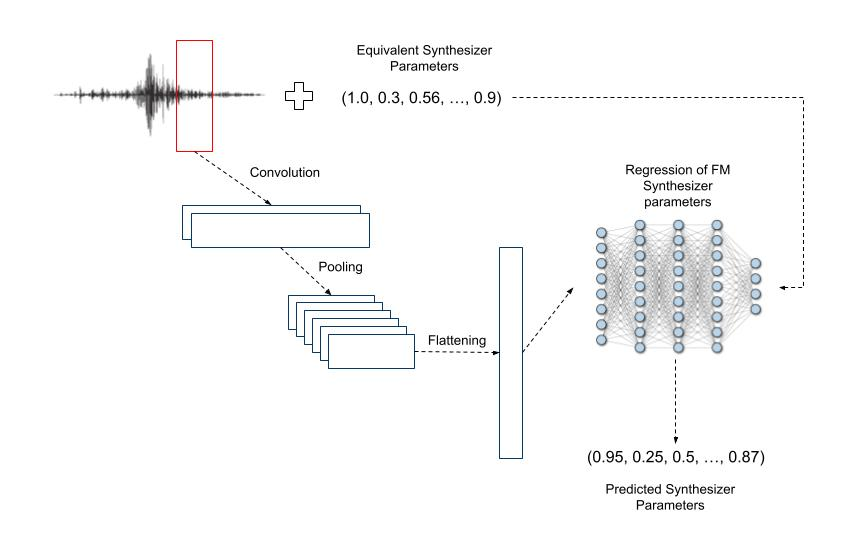
\includegraphics[width=\linewidth]{figs/cnn_simple_training.jpg}
%     \caption{The overall training scheme.}
%     \Description{The overall training scheme.}
%     \label{fig:cnn}
% \end{figure}

\subsection{Evaluating the Model} \label{sec:evaluation_method}

After training the CNN, a new dataset is used to evaluate the model’s ability to re-synthesize real instruments by calculating specific metrics focused on the FM synthesizer’s capacity to reproduce the same timbres.

\begin{figure}[h]
    \centering
    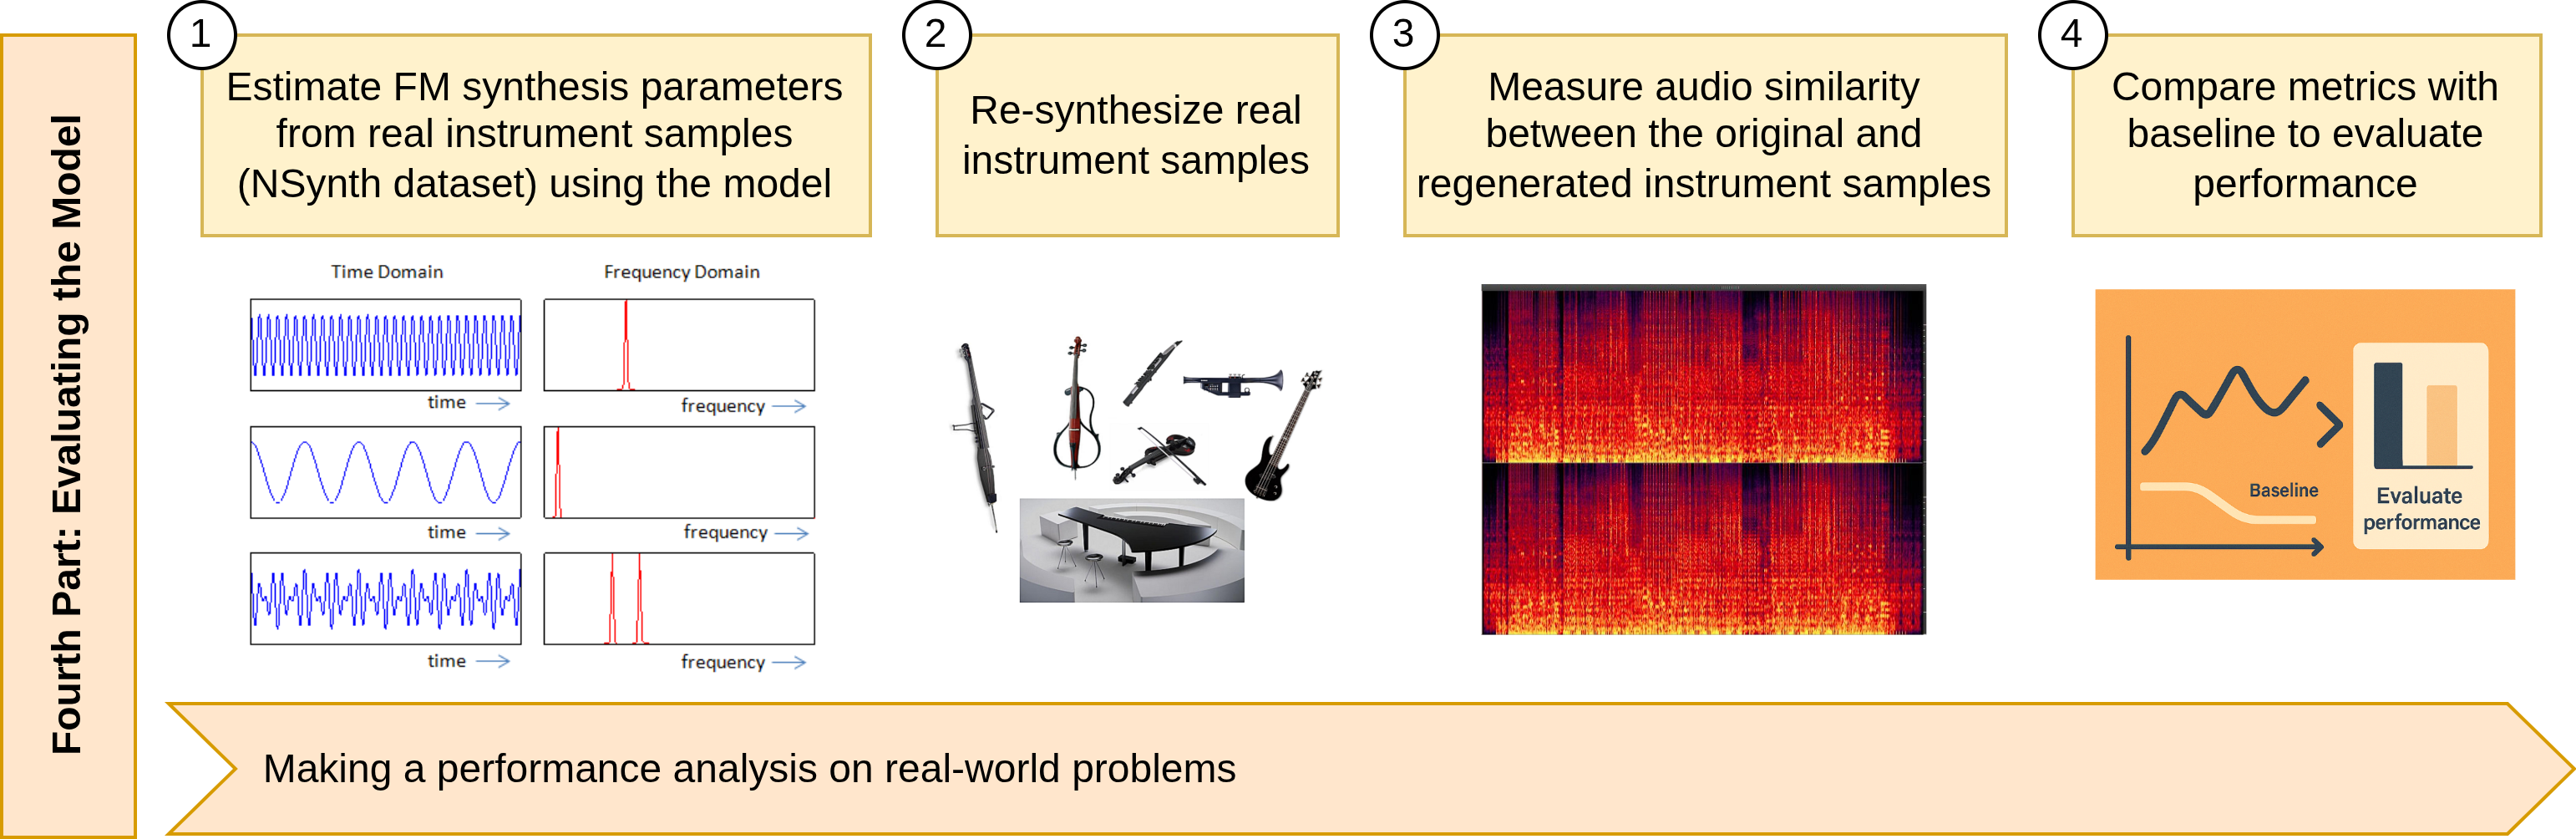
\includegraphics[width=1\columnwidth]{figs/fourth_part.png}
    \caption{Results evaluation.}
    \label{fig:met3}
\end{figure}

The NSynth dataset, part of Google’s Magenta project, contains numerous real instrument samples, including both acoustic and electronic instruments, as well as some synthetic sounds generated by professional synthesizers. This dataset has a configuration similar to that of the generated one used for training, and its main purpose is to evaluate the model’s generalization capabilities, since the model has never encountered it before.

Only the test set of the NSynth dataset will be used, with the following characteristics:

\begin{itemize}
    \item 4,096 samples.
    \item 4 seconds in duration.
    \item Monophonic samples (1-channel audio).
    \item 16 kHz audio sample rate.
    \item 11 instrument families.
    \item Pitches ranging from 27.5 Hz to 4,186.01 Hz.
    \item The envelope includes a sustain of up to 3 seconds and a decay of 1 second.
\end{itemize}

The basic idea is to use the NSynth test samples as input to the model and, after predicting the synthesizer parameters, employ the implemented synthesizer to re-synthesize all samples. Finally, audio comparison metrics are calculated between each input and its corresponding generated sound, based on the proposed evaluation measures:

\begin{itemize}
    \item FFT distance: Used to compare the frequency components present in an audio signal.
    \item STFT distance: Used to compare the variation of frequency components over time.
    \item Log-mel-spectrogram distance: Used for a similar purpose as FFT distance, but typically models human cognitive pitch perception more accurately.
\end{itemize}

However, before using the predicted parameters as input to the synthesizer, a simple function was applied to approximate each ratio parameter to the nearest discrete ratio, according to the common behavior of musical harmonics (the same set of ratios used to randomize 90\% of the generated dataset). Furthermore, some clipping operations were also applied to enforce the same limits imposed on the randomly generated dataset, such as maximum and minimum values for beta parameters.

In order to achieve a good evaluation, the proposed metrics were also used to compare each NSynth audio with a baseline, which consists of a pure sinusoidal signal, with a frequency of 440 Hz (i.e., the A4 note, which is used as a reference to tune the majority of instruments).

\section{Experimental Results and Discussion}  \label{sec:experiments}

This section presents the final results of the model, considering both the training metrics and the audio comparision metrics. The former is used to evaluate the model’s ability to learn the entire parameter space, while the latter assesses its generalization capabilities, particularly its ability to emulate real instruments.

\subsection{Training Results}

The training and validation results are shown in the following table, which summarizes the last five epochs of training:

\begin{table} \small
  \caption{Training and Validation Metrics by Epoch}
  \label{tab:train_val_metrics_2}
  \begin{tabular*}{\columnwidth}
    {@{\extracolsep{\fill}}c|ccc|ccc}
    \toprule
    \multirow{2}{*}{Epoch} & \multicolumn{3}{c|}{Train} & \multicolumn{3}{c}{Validation} \\
     & Loss & MAE & MSE & Loss & MAE & MSE \\
    \midrule
    70 & 0.603 & 0.527 & 0.545 & 0.622 & 0.517 & 0.562 \\
    71 & 0.601 & 0.526 & 0.542 & 0.637 & 0.520 & 0.569 \\
    72 & 0.605 & 0.526 & 0.545 & 0.621 & 0.516 & 0.565 \\
    73 & 0.602 & 0.524 & 0.541 & 0.625 & 0.522 & 0.568 \\
    74 & 0.611 & 0.528 & 0.548 & 0.625 & 0.520 & 0.563 \\
    \bottomrule
  \end{tabular*}
\end{table}

Regarding the loss evolution across epochs, consider the following graphs:

\begin{figure}[h]
 \centering
 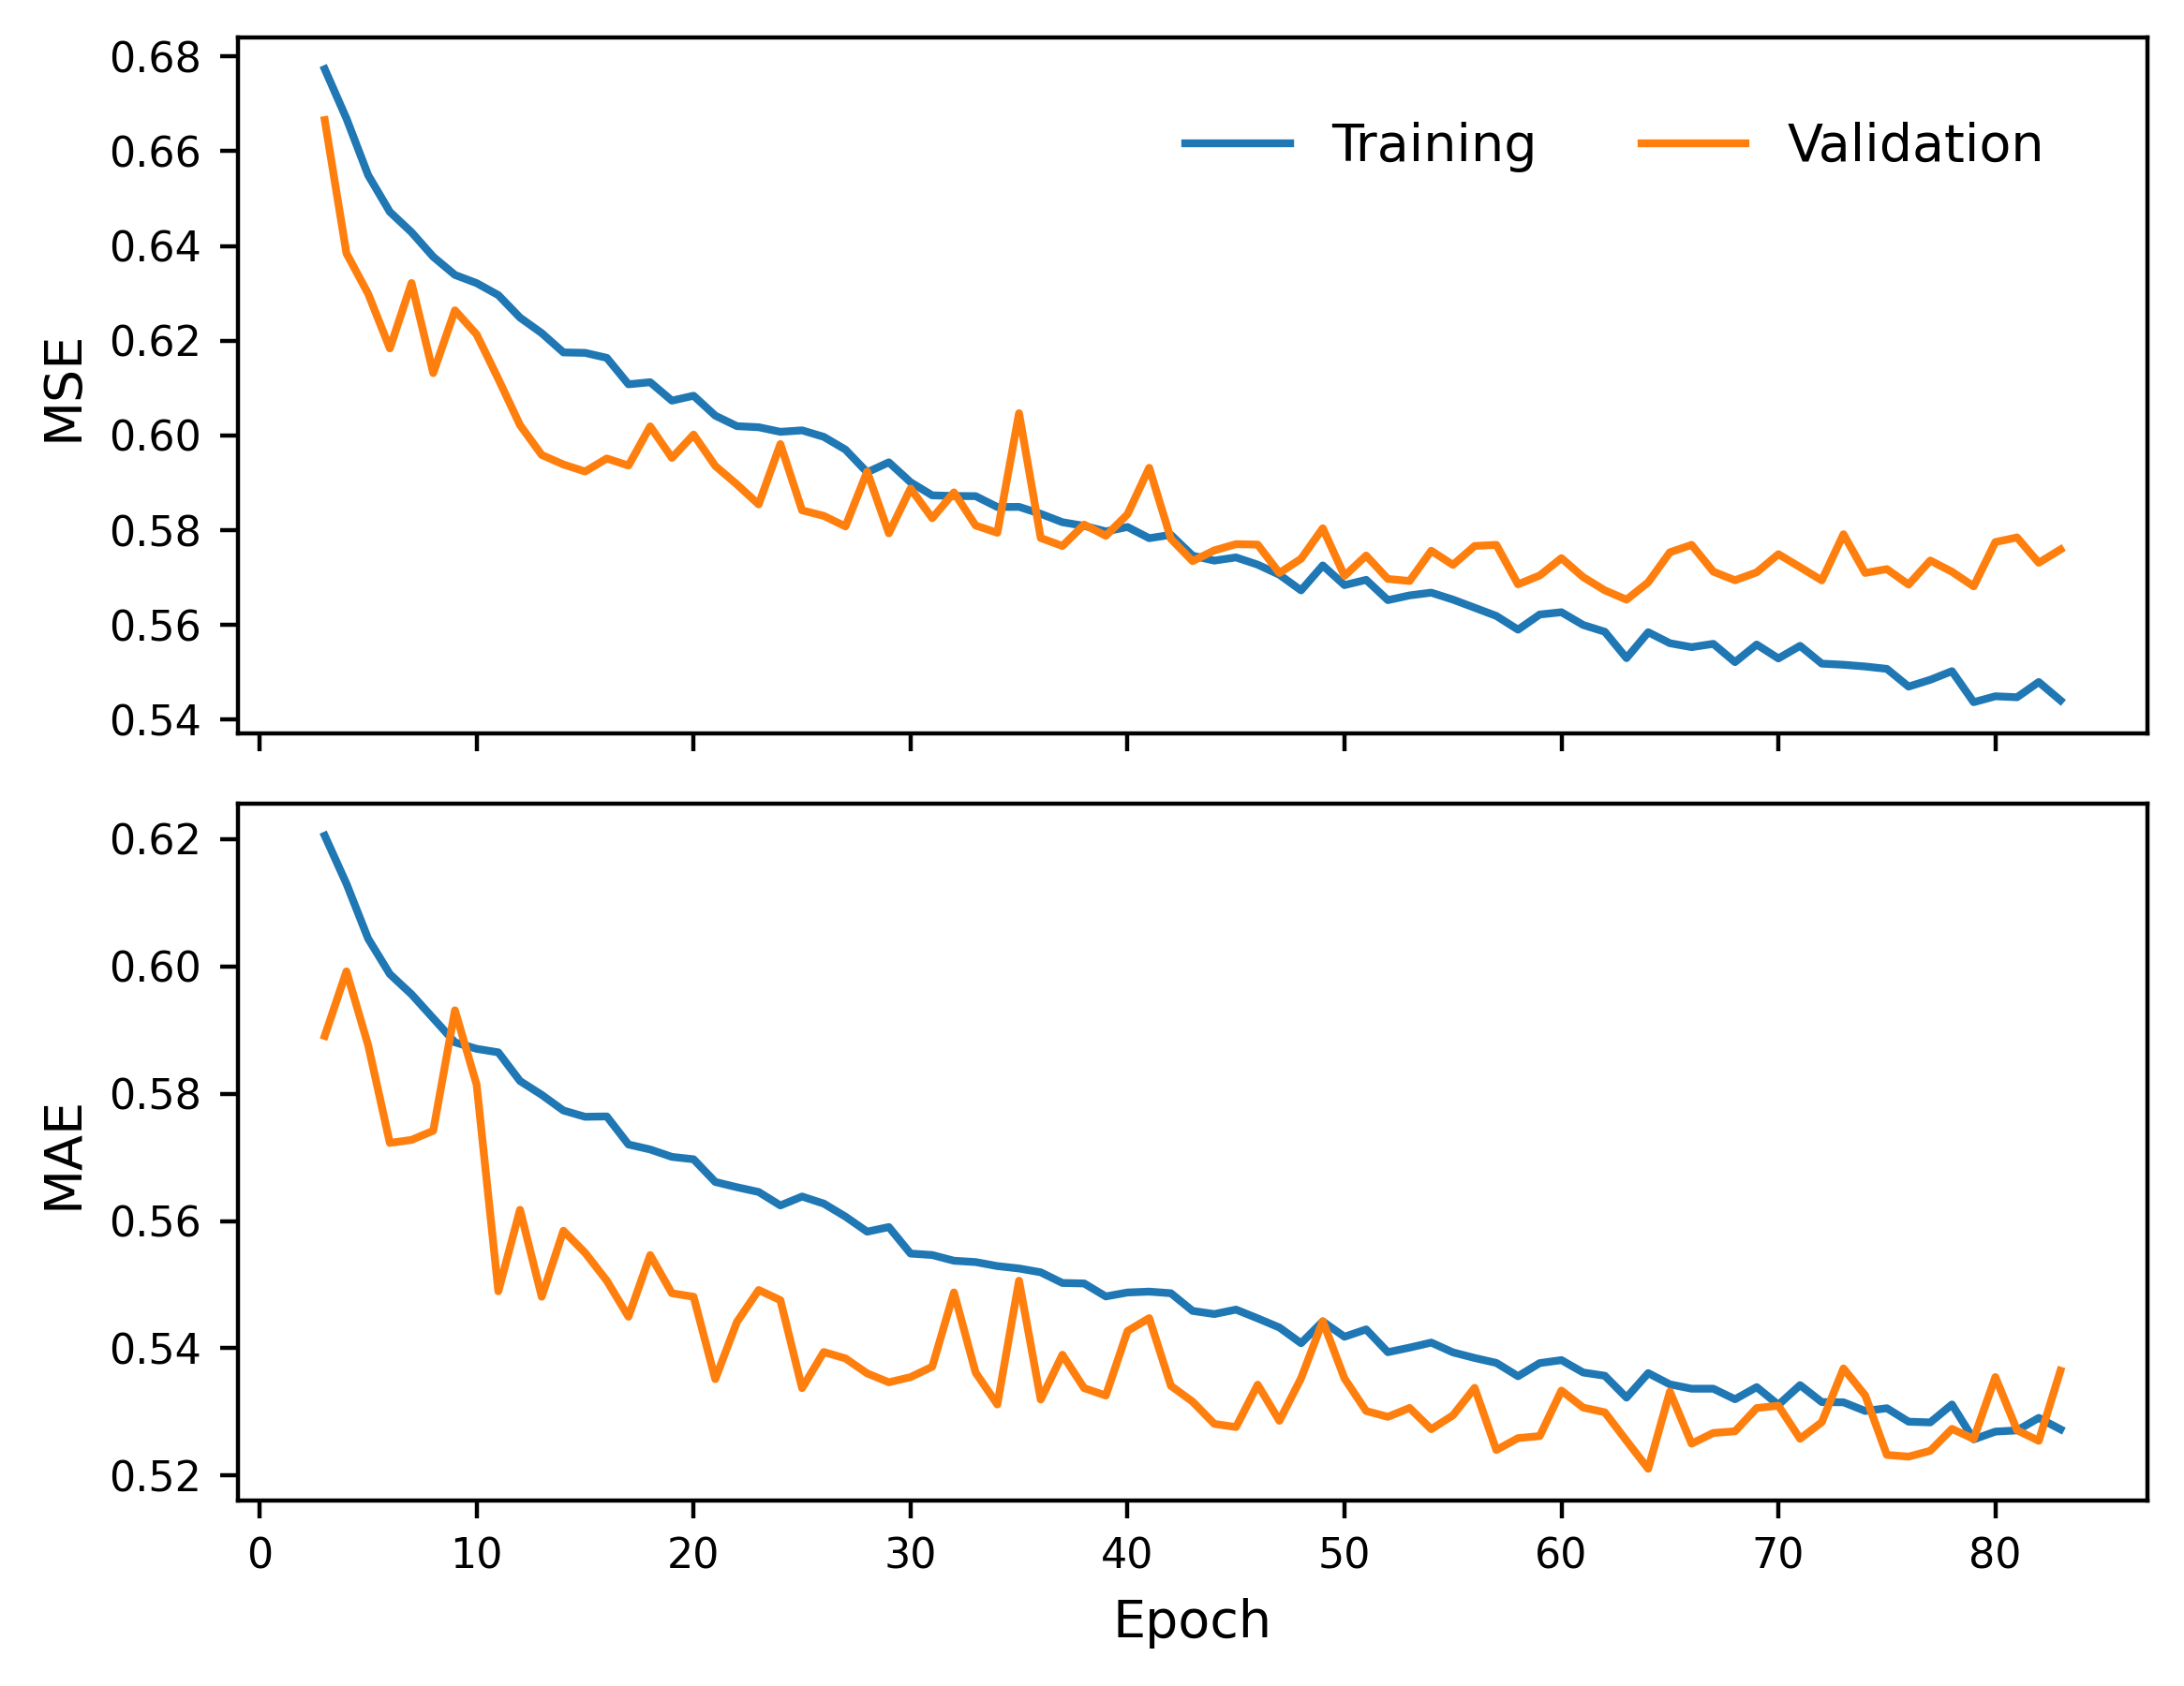
\includegraphics[width=\linewidth]{figs/mae_mse_evolution.png}
 \caption{Evolution of MAE and MSE during training.}
\end{figure}


% \begin{figure}[h]
%  \centering
%  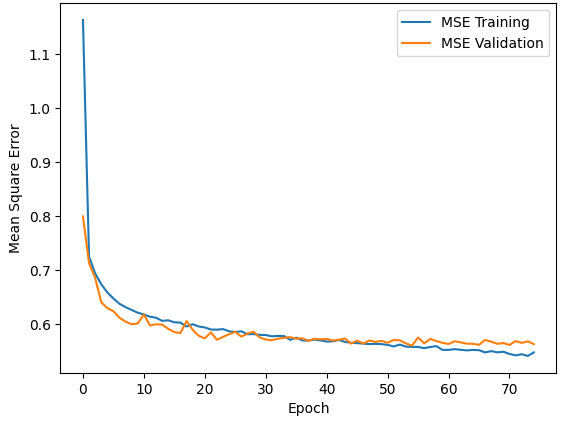
\includegraphics[width=\linewidth]{figs/mse_evolution.png}
%  \caption{Evolution of MSE during training.}
%  \Description{Evolution of MSE during training.}
% \end{figure}

% \begin{figure}[h]
%  \centering
%  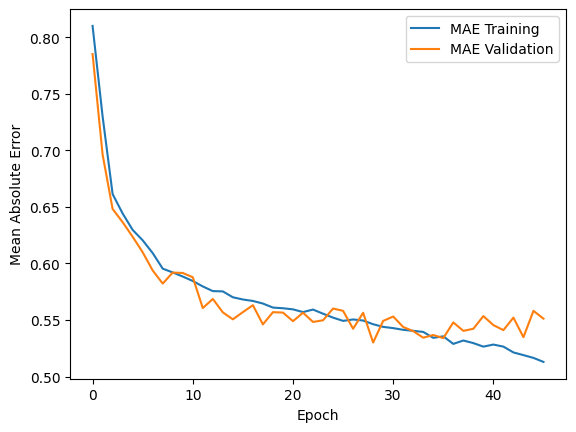
\includegraphics[width=\linewidth]{figs/mae_evolution.png}
%  \caption{Evolution of MAE during training.}
%  \Description{Evolution of MAE during training.}
% \end{figure}

After the training, still using a splitted part of the synthetic dataset, the test results was calculated. The predicted values were transformed back to the original space, and the results indicates:

\begin{itemize}
    \item \textbf{Mean Absolute Error (MAE):} 6.488
    \item \textbf{Mean Squared Error (MSE):} 1410.097
    \item \textbf{Root Mean Squared Error (RMSE):} 37.551
\end{itemize}

And, these values demonstrate the model’s ability to reproduce the synthetic parameters.

\subsection{Audio Comparision Results}

%Then, the results can be seen in the following:

%Comparison of Resynthesis and Baseline in terms of three different metrics. 

%\begin{table} \small % desvios nas linhas debaixo
  %\caption{Comparision between Resynthesis and Baseline in terms of three metrics. The values represent average and standard deviation (between parentheses). Improvement shows positive gains of Resynthesis over Baseline.}

%    \caption{Average and standard deviation (between parentheses) values for Resynthesis and Baseline.}%, with Improvement \%).}
%   \label{tab:metrics}
% \begin{tabular*}{\columnwidth}
% 	{@{\extracolsep{\fill}}lccc}
%     \toprule
%     Metric & Resynthesis & Baseline & Improvement (\%) \\
%     \midrule
%     \multirow{2}{*}{STFT}  & 2366.4 & 7290.4  & \multirow{2}{*}{67.540}  \\
%       &  (1132.2) & (434.87)  & \\
%     %Log Mel (raw)
%     \multirow{2}{*}{Log Mel (raw)} & 138.73  & 184.87 & \multirow{2}{*}{24.960} \\
%        &  (47.013) & (30.136) & \\
%     %Log Mel (normalized)
%     \multirow{2}{*}{Log Mel (normalized)} & 0.0086 & 0.0115 & \multirow{2}{*}{24.930} \\
%     &  (0.0029)  & (0.0019) & \\
%     \bottomrule
%   \end{tabular*}
% \end{table}

As presented in Section~\ref{sec:evaluation_method}, after training, the model’s generalization capabilities were tested through a process of re-synthesizing the NSynth dataset. The performance was evaluated by comparing the audio distance metrics between the original samples and the baseline samples with those between the re-synthesized samples and the original ones:

\begin{table} \small % desvios nas colunas
  \caption{Comparison between Resynthesis and Baseline with Improvement \% (considering mean and standard deviation).}
  \label{tab:metrics}
\begin{tabular*}{\columnwidth}
	{@{\extracolsep{\fill}}lccccc}
    \toprule
    Metric & Resynthesis & STD & Baseline & STD & Tuning (\%) \\
    \midrule
    FFT  & 12649.9 & 6208.1 & 33508.8 & 1887.36  & 62.270 \\
    STFT  & 2366.4 & 1132.2  & 7290.4 & 434.87  & 67.540 \\
    %Log Mel (raw)
    Log Mel (r) & 138.73 & 47.013 & 184.87 & 30.136 & 24.960 \\
    %Log Mel (normalized)
    Log Mel (n) & 0.0086 & 0.0029  & 0.0115 & 0.0019 & 24.930 \\
    \bottomrule
  \end{tabular*}
  \label{tab:metrics}
\end{table}

% \begin{table}
%   \caption{Comparison of Means (Resynthesis vs Baseline, with Improvement \%)}
%   \label{tab:metrics_means_updated}
%   \begin{tabular}{lccc}
%     \toprule
%     Metric & Resynthesis & Baseline & Improvement (\%) \\
%     \midrule
%     FFT   & 12649.920 & 33508.780 & 62.27 \\
%     STFT  & 2366.424  & 7290.362  & 67.54 \\
%     Log Mel (raw) & 138.732 & 184.872 & 24.96 \\
%     Log Mel (normalized) & 0.00860 & 0.01146 & 24.93 \\
%     \bottomrule
%   \end{tabular}
% \end{table}

% \begin{table}
%   \caption{Comparison of Standard Deviations (Resynthesis vs Baseline)}
%   \label{tab:metrics_std_updated}
%   \begin{tabular}{lcc}
%     \toprule
%     Metric & Resynthesis & Baseline \\
%     \midrule
%     FFT   & 6208.149 & 1887.364 \\
%     STFT  & 1132.152 & 434.867  \\
%     Log Mel (raw) & 47.013 & 30.136 \\
%     Log Mel (normalized) & 0.00292 & 0.00187 \\
%     \bottomrule
%   \end{tabular}
% \end{table}

Note that the Log Mel metric was compared, including a normalized version, which is obtained by dividing the raw Log Mel value by the product of the number of Mel bands and the time window quantity.

% Another important insight can be obtained from a histogram representation of the Log-Mel distances, shown in Figure~\ref{fig:histo}. \basg{qual insight? se nao for explicar o que a figura diz, melhor tirar}

% \begin{figure}[h]
%  \centering
%  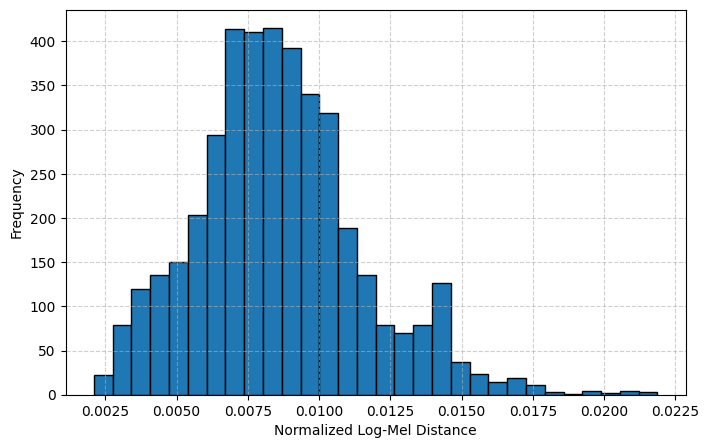
\includegraphics[width=\linewidth]{figs/historgram_quality.png}
%  \caption{Distribution of Normalized Log-Mel Distance.}
%  \label{fig:histo}
% \end{figure}

Furthermore, to facilitate a better understanding, the metrics were also compared by grouping the dataset by instrument family. This allows for the evaluation of the model's performance on different classes of sounds. Tables~\ref{tab:avg_metrics_groups} and \ref{tab:stdev_metrics_groups} show the average and standard deviation values, respectively. We can note that the top three best results were obtained for keyboard, guitar, and mallet families.


\begin{table} \small
  \caption{Comparison of Average by Instrument Group}
  \label{tab:means_by_group_updated}
  \begin{tabular}{lcccc}
    \toprule
    Group & FFT & STFT & Log Mel (raw) & Log Mel (norm) \\
    \midrule
    bass     & 11232.7 & 2144.32 & 135.610 & 0.00841 \\
    brass    & 14371.1 & 2682.95 & 167.617 & 0.01039 \\
    flute    & 14611.3 & 2872.69 & 141.819 & 0.00879 \\
    guitar   & 9692.0  & 1867.47 & 119.853 & 0.00743 \\
    keyboard & 9619.3  & 1772.92 & 119.529 & 0.00741 \\
    mallet   & 8085.8  & 1632.45 & 120.610 & 0.00748 \\
    organ    & 18360.1 & 3453.13 & 166.433 & 0.01032 \\
    reed     & 12740.0 & 2267.08 & 140.701 & 0.00872 \\
    string   & 12883.7 & 2390.65 & 139.365 & 0.00864 \\
    vocal    & 31028.9 & 5271.26 & 212.646 & 0.01319 \\
    \bottomrule
  \end{tabular}
  \label{tab:avg_metrics_groups}
\end{table}

\begin{table} \small
  \caption{Comparison of Standard Deviations by Instrument Group}
  \label{tab:std_by_group_updated}
  \begin{tabular}{lcccc}
    \toprule
    Group & FFT & STFT & Log Mel (raw) & Log Mel (norm) \\
    \midrule
    bass     & 5271.64 & 931.050 & 43.094 & 0.00267 \\
    brass    & 3934.39 & 949.146 & 50.102 & 0.00311 \\
    flute    & 3711.78 & 769.482 & 36.122 & 0.00224 \\
    guitar   & 3805.30 & 716.923 & 38.010 & 0.00236 \\
    keyboard & 3024.45 & 507.672 & 34.145 & 0.00212 \\
    mallet   & 2304.33 & 437.872 & 38.022 & 0.00236 \\
    organ    & 3418.07 & 818.277 & 47.884 & 0.00297 \\
    reed     & 4205.59 & 905.286 & 46.032 & 0.00285 \\
    string   & 4696.61 & 889.743 & 35.951 & 0.00223 \\
    vocal    & 8218.04 & 1672.940 & 56.507 & 0.00350 \\
    \bottomrule
  \end{tabular}
  \label{tab:stdev_metrics_groups}
\end{table}

% \begin{table} \small
%   \caption{Comparison of Standard Deviations by Instrument Group}
%   \label{tab:std_by_group_updated}
%   \begin{tabular}{lcccc}
%     \toprule
%     Group & FFT & STFT & Log Mel (raw) & Log Mel (norm) \\
%     \midrule
%     bass     & 5271.640 & 931.050 & 43.094 & 0.00267 \\
%     brass    & 3934.388 & 949.146 & 50.102 & 0.00311 \\
%     flute    & 3711.774 & 769.482 & 36.122 & 0.00224 \\
%     guitar   & 3805.303 & 716.923 & 38.010 & 0.00236 \\
%     keyboard & 3024.448 & 507.672 & 34.145 & 0.00212 \\
%     mallet   & 2304.329 & 437.872 & 38.022 & 0.00236 \\
%     organ    & 3418.068 & 818.277 & 47.884 & 0.00297 \\
%     reed     & 4205.592 & 905.286 & 46.032 & 0.00285 \\
%     string   & 4696.608 & 889.743 & 35.951 & 0.00223 \\
%     vocal    & 8218.038 & 1672.940 & 56.507 & 0.00350 \\
%     \bottomrule
%   \end{tabular}
% \end{table}


\section{Conclusion} \label{sec:conclusion}

This work aimed to develop and evaluate a technique capable of achieving two primary objectives: re-synthesizing the sounds of real musical instruments and exploring the synthesizer’s parameter space in a randomized manner to assess the model’s generalization capacity. The proposed convolutional neural network (CNN) model demonstrated strong performance in both aspects, effectively reproducing real instrument timbres and showing satisfactory generalization when exposed to unseen parameter configurations. The re-synthesized audios, when compared to the original samples from the NSynth dataset, confirmed the model’s ability to approximate realistic timbral characteristics, while maintaining consistent performance across different instrument families. The stability of the normalized log-mel metric across all categories suggests that the model is not overly biased toward specific timbral structures, reinforcing its robustness and flexibility. These results validate the initial hypothesis that CNNs are highly efficient in extracting relevant spectral and temporal features from audio signals, and that randomized dataset generation can effectively guide the learning process, enabling a level of control over FM synthesis parameters sufficient to emulate real-world sounds.

Despite these promising outcomes, the approach presents some limitations that delineate directions for future research. First, the use of a dataset restricted to musical instruments limits the generalization potential of the system; therefore, future experiments should incorporate more diverse sound sources, such as environmental or synthetic noises, to enhance creative applicability. Additionally, the adoption of a single linear ADSR envelope constrained the diversity of synthesized dynamics, indicating that broader variations should be implemented to better model non-instrumental or abstract sound categories. Another limitation concerns the exploration of FM synthesis algorithms, as only two were tested, and a single configuration yielded satisfactory results; expanding this investigation to include more complex operator topologies could significantly improve the synthesis flexibility.

Future work should thus focus on testing alternative neural architectures, such as autoencoders, to improve feature representation and generalization, as well as combining CNN-based feature extraction with other strategies found in the literature, including the use of STFT-based regression inputs or perceptually informed loss functions such as the log-mel metric. Moreover, the application of AutoML techniques could optimize the regression stage of the pipeline, potentially enhancing the model’s predictive performance. Finally, retraining the model using a professional FM synthesizer implementation would provide a more realistic framework for evaluation and deployment, advancing the state of neural sound synthesis and broadening its relevance for both academic research and creative audio production.

\balance

% \section{Conclusion} \label{sec:conclusion}

% As proposed in the introduction of this work, there are two main goals to achieve with this technique: the first is to re-synthesize the sounds of real instruments, and the second is to explore the parameter space in a randomized way, testing whether the model can generalize the results. This generalization is a strong indication that the model can guide the synthesizer to reproduce arbitrary sounds.

% As shown in the results, the CNN model demonstrated good generalization ability and also showed strong performance in the re-synthesis of real instruments, as evidenced by the audio comparison metrics between the NSynth dataset and the corresponding re-synthesized audio.

% Furthermore, the results indicate that the model is not extremely biased toward specific instrument families. As presented in the previous section, the normalized log-mel metric remained within a reasonable range across all instrument families, and the difference between the best and worst cases was not excessively high.

% The proposed approach clearly shows that both pillars of the initial hypothesis were valid:

% \begin{itemize}
%     \item CNNs are highly effective for feature extraction from instrument audio samples.
%     \item The approach of generating a randomized dataset, aiming to cover a wide area of the parameter space, was efficient in achieving reasonable control over a specific FM synthesizer.
% \end{itemize}

% However, this work also has clear limitations that should be highlighted, which at the same time represent opportunities for future research:

% \begin{itemize}
%     \item \textbf{Generic dataset:} Adopt a new dataset composed of generic audio samples, not limited to musical instruments (e.g., bells, horns, bird calls, etc.), which could serve as inspiration for musicians.
%     \item \textbf{Broader ADSR envelope variations:} Since the main goal was related to real instrument re-synthesis, and the test dataset (NSynth) is composed of such sounds, only a standard linear ADSR envelope was implemented. While sufficient for this purpose, it would certainly not be adequate for a more generic dataset.
%     \item \textbf{Exploring more FM synthesis algorithms:} During the experiments, only two FM algorithms were evaluated, and only one produced good results (the one with three serial operators and two parallel operators, which was used for all reported results). However, professional FM synthesizers typically allow arbitrary operator configurations, which could be explored further.
% \end{itemize}

% \subsection{Future Work}

% To highlight future research opportunities, the following directions appear most promising:

% \begin{itemize}
%     \item Explore the use of more generic datasets.
%     \item Implement and evaluate a wider range of ADSR envelopes and FM algorithms.
%     \item Investigate less straightforward neural network architectures, testing whether feature extraction through core representation (e.g., autoencoder networks) could be effective for generic datasets.
%     \item Combine approaches from related works: for example, using the STFT of each sample as input to the regression stage of the network (\textcite{claesson2021resynthesis}) alongside CNN-based feature extraction from raw signals, or applying the log-mel metric directly in the loss function, as in DDX7 (\textcite{steinmetz2022ddx7}).
%     \item Experiment with AutoML techniques after CNN feature extraction, as a way to improve the regression stage of the model. In this context, the autoencoder hypothesis could also be used to pre-train the CNN independently.
%     \item Adopt a professional FM synthesizer implementation (with the necessary permissions) to re-train the entire model.
% \end{itemize}

% \begin{acks}
% This work is supported by \textit{Coordenação de Aperfeiçoamento de Pessoal de Nível Superior}~(CAPES), \textit{Conselho Nacional de Desenvolvimento Científico e Tecnológico}~(CNPq), grants 406417/2022-9, 102475/2024-5, and 312209/2022-3, and \textit{Fundação de Amparo à Pesquisa do Estado de São Paulo}~(FAPESP), grant 2020/09835-1~(CPA IARA). 
% \end{acks}


%%
%% Print the bibliography
%%
\printbibliography


\end{document}
\endinput
%% End of file `sample-sigconf-biblatex.tex'.
